\documentclass[12pt,a4paper,openright]{book}
\title{\Huge DISEÑO}
\date{\today}
\author{Grupo PMC}
\pagestyle{plain}
\usepackage[spanish]{babel}
\usepackage[top=2.5cm, bottom=2.5cm, left=3cm, right=3cm]{geometry}
\setlength{\parskip}{0.25cm} %edicion de espaciado
\setlength{\parindent}{0cm} %edicion de sangría
\clubpenalty=10000 %líneas viudas NO
\widowpenalty=10000 %líneas viudas NO

\usepackage{graphicx}
\graphicspath{{./fotos/}}
\usepackage{ntheorem}[thmmarks]	% paquete de formateo de entornos matemáticos
\usepackage{listings}
\usepackage{ulem}
\usepackage[explicit]{titlesec} %Formato de capitulos y secciones
\usepackage{hyperref} %Hipervínculos y referencias

\hypersetup{
	colorlinks = true,
	linkcolor = blue
}

\urlstyle{same}

\newcommand{\defaultformat}{
	\titleformat{\chapter}[display]{\centering\normalfont\huge\bfseries}{}{0pt}{\Huge \uppercase{##1}}[\titlerule]
    \titleformat{\section}{\normalfont\Large\bfseries}{}{0pt}{##1}
    \titleformat{\subsection}{\normalfont\large\bfseries}{}{0pt}{\uline{##1}}
    \titleformat{\subsubsection}{\normalfont\normalsize\bfseries}{}{0pt}{##1}
}

\theoremstyle{break}
\theoremheaderfont{\normalfont\bfseries}
\theorembodyfont{}
\theoremseparator{\vspace{0.2cm}}
\theorempreskip{\topsep}
\theorempostskip{\topsep}
\theoremindent0cm
\theoremnumbering{arabic}
\theoremsymbol{}
\theoremprework{\vspace{0.2cm}}
\theorempostwork{\vspace{0.2cm}}
    \newtheorem*{sprint}{Sprint}
    
\usepackage[dvipsnames,usenames]{xcolor} %activar e incluir colores
    \definecolor{comentarios}{RGB}{186,196,200}
    \definecolor{words}{RGB}{87,35,100}

\lstset{
    language=Java,
    basicstyle=\scriptsize\ttfamily,
    numbers=left,
    numberstyle=\tiny,
    frame=tb,
    tabsize=4,
    columns=fixed,
    showstringspaces=false,
    showtabs=false,
    keepspaces,
    commentstyle=\color{comentarios},
    keywordstyle=\color{words}
}

\begin{document}
\defaultformat
\maketitle
\setcounter{tocdepth}{3}
\setcounter{secnumdepth}{3}
\tableofcontents

\chapter{Diseño y evolución de las Historias de Usuario}

\subsection{Como usuario quiero poder jugar a Rolit siguiendo un conjunto mínimo de normas}

\begin{sprint}[1]

\begin{center}
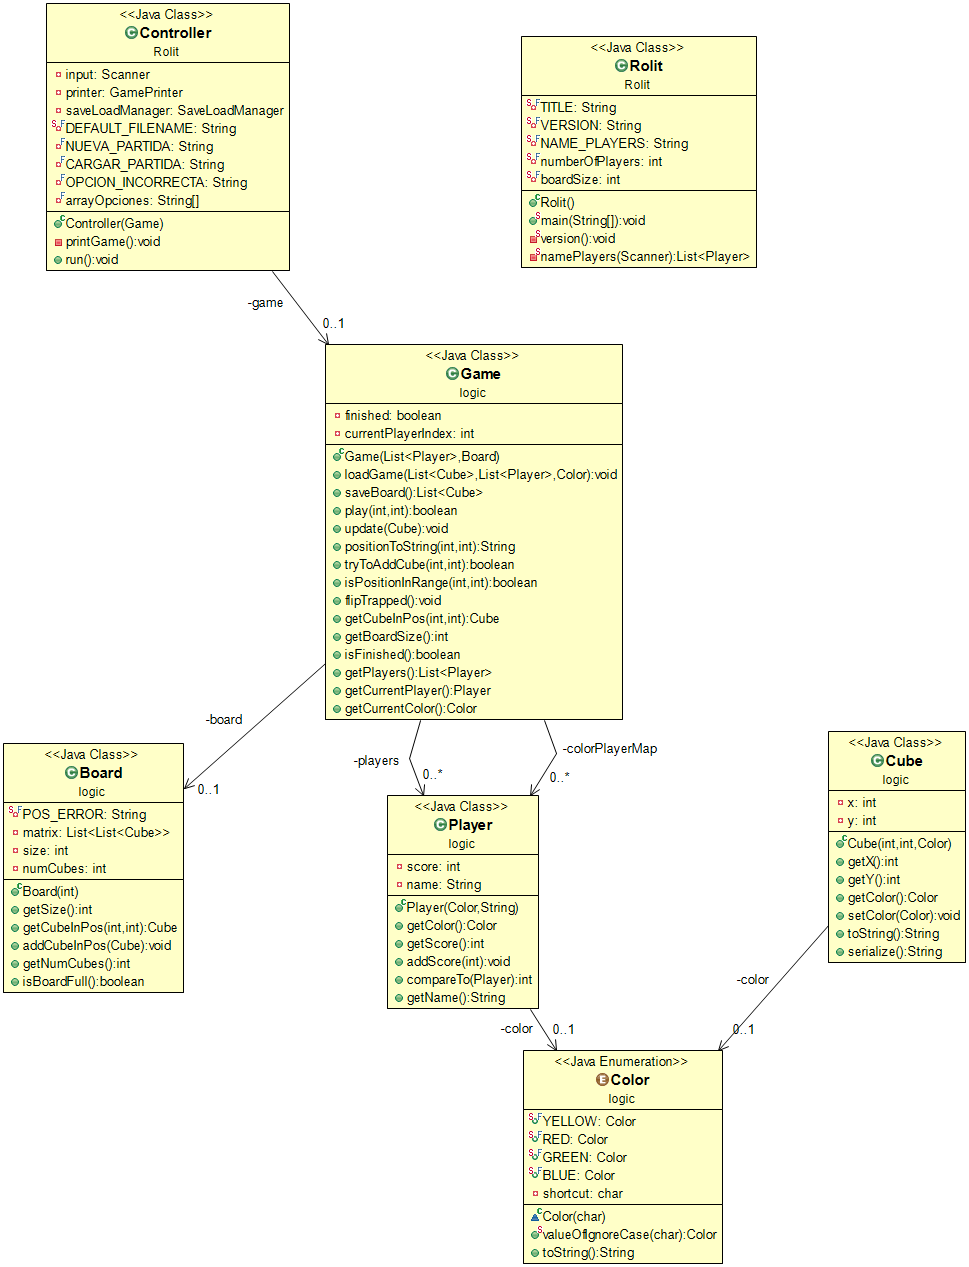
\includegraphics[scale=0.3]{logicS1.png}
\end{center}
Esta es la versión más básica de Rolit.

El tablero es un cuadrado 8x8. Esto se hace por medio de una constante llamada \texttt{boardSize}, dentro de la clase \texttt{Rolit} y cuyo valor era trivialmente 8. 

Hay una cantidad invariable de 4 jugadores cuyos colores son: amarillo, rojo, verde y azul. El enumerado \texttt{Color} facilita la gestión de dicha tarea, ya que cada cubo y cada jugador tienen asignado un \texttt{Color}, como bien muestra el diagrama de clases. 

Aunque la intención final es que los cubos sean redondos, en esta versión de Rolit decidimos no implementarlo aún. Por ello el tablero se muestra gracias a \texttt{GamePrinter} como una matriz 8x8 en la que los cubos están representados por la letra inicial del color, tal y como se muestra en la imagen inferior.
\begin{center}
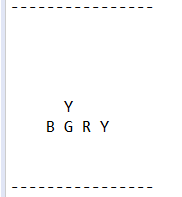
\includegraphics[scale=0.8]{Board.png}
\end{center}

Los jugadores están almacenados en una lista de \texttt{Player} y en un mapa de \texttt{Color, Player} en la clase \texttt{Game}. Esto es necesario para el funcionamiento del método \texttt{update(Cube)}, que es el encargado de llevar a cabo las siguientes tareas:
\begin{itemize}
\item Solo se puede colocar un cubo en una casilla vacía adyacente a una ya ocupada (ver imagen inferior), excepto el primer cubo que se pone donde se desee.
\begin{center}
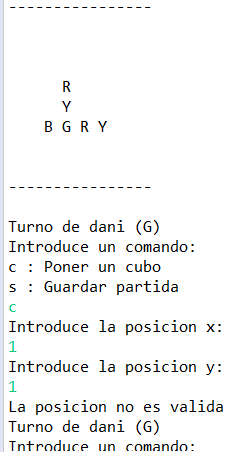
\includegraphics[scale=0.8]{pos-no-validaS1.png}
\end{center}

\item Cuando se coloca un cubo, se cambian de color todos los que quedan atrapados en las direcciones válidas. Un cubo se dice atrapado cuando se encuentra en la línea que une un cubo recién puesto con otro del mismo color y las direcciones válidas son las líneas rectas dadas por alguna de las casillas adyacentes.
\begin{center}
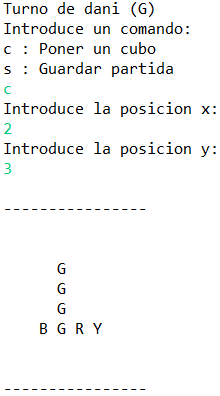
\includegraphics[scale=0.8]{atrapadaaaaaaaas.png}
\end{center}

\item En cada turno un jugador pone un único cubo y se pasa de turno al siguiente jugador después de haber cambiado de color a los posibles cubos atrapados.

\item El juego acaba cuando el tablero se llena completamente.
\end{itemize} 

Para poder entender el método \texttt{update(Cube)} de una forma más simple hay que contextualizarlo primero. El \texttt{main()} está dentro de la clase \texttt{Rolit} y es el encargado de instanciar \texttt{Controller, Game y Board}, así como de crear la lista de \texttt{Player}.
\begin{center}
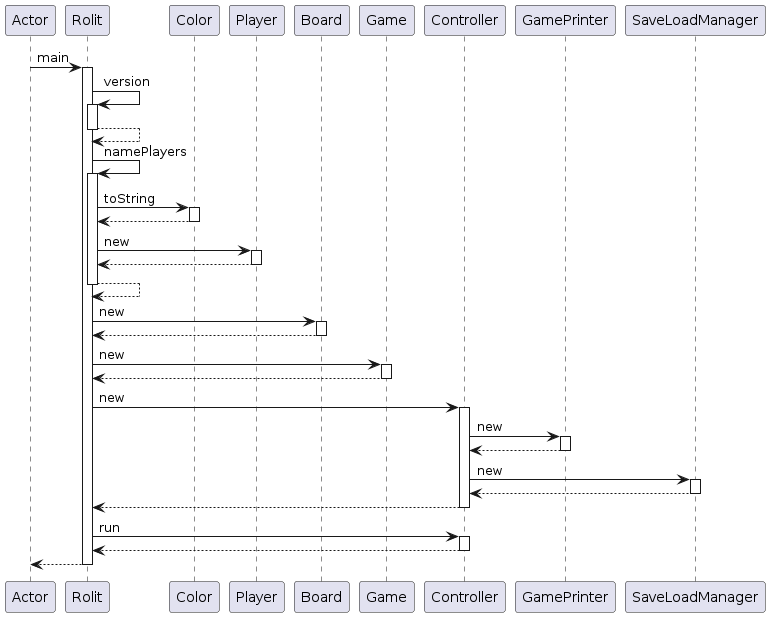
\includegraphics[scale=0.28]{mainS1.png}
\end{center}

Por otro lado el método \texttt{run()} se encarga de gestionar la ejecución global del juego, el cual será ejecutado hasta que haya terminado, es decir, cuando el tablero se esté completamente lleno. Esto se gestiona por medio de un bucle cuya condición es \texttt{!game.isFinished()}, esta función actúa como un getter del atributo privado \texttt{finished} de la clase \texttt{Game}, como bien se puede apreciar en el diagrama de clases. Por último, se mostrará un ranking, por medio de \texttt{GamePrinter} a través del método \texttt{showRanking()}, que muestra una lista de los jugadores ordenados según su atributo \texttt{score}, es decir, ganará el jugador con más puntos.
\begin{center}
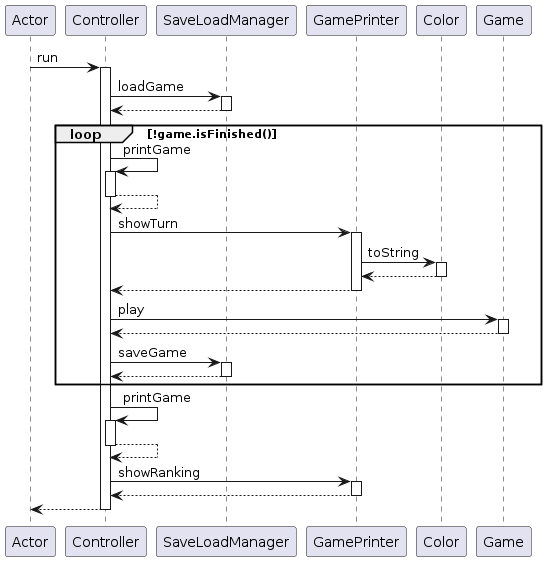
\includegraphics[scale=0.28]{controller-runS1.png}
\end{center}

El método \texttt{play()} comprueba en primer lugar que la posición en la que se quiere colocar el cubo es válida. En caso afirmativo se crea un \texttt{Cube} y se llama al método \texttt{update()}, al que queríamos llegar desde un comienzo y podríamos considerar núcleo de la lógica de Rolit.
\begin{center}
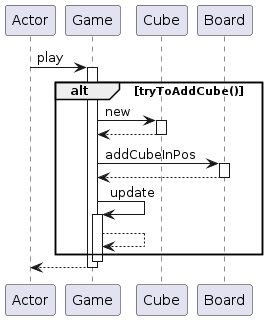
\includegraphics[scale=0.35]{play-game.png}
\end{center}

Como bien se puede observar en el diagrama de secuencias inferior, el método
\texttt{update()} de Game  es el encargado de cambiar de color todos los cubos que quedan atrapados en las direcciones válidas, así como de actualizar el atributo \texttt{finished} si la partida haya acabado, en otro caso avanza el turno para que cada jugador solo colocar un cubo en cada turno.
\begin{center}
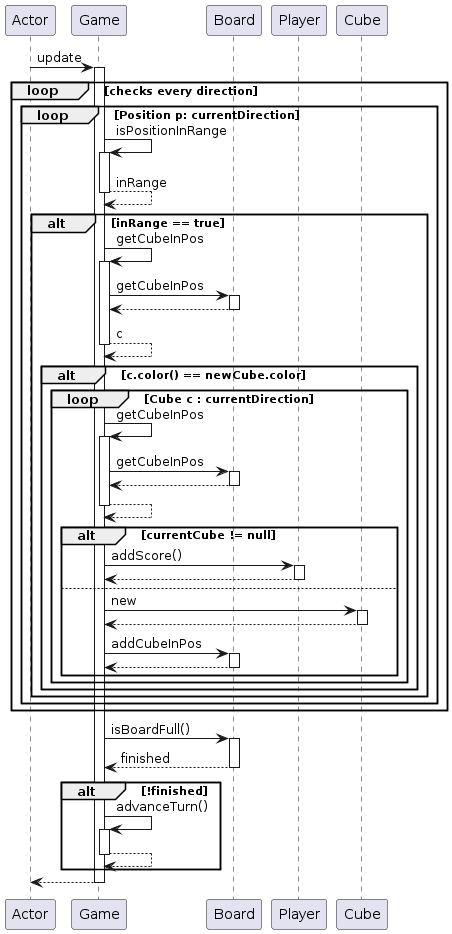
\includegraphics[scale=0.35]{updateGameS1.png}
\end{center}

\end{sprint}


\begin{sprint}[2]

\begin{center}
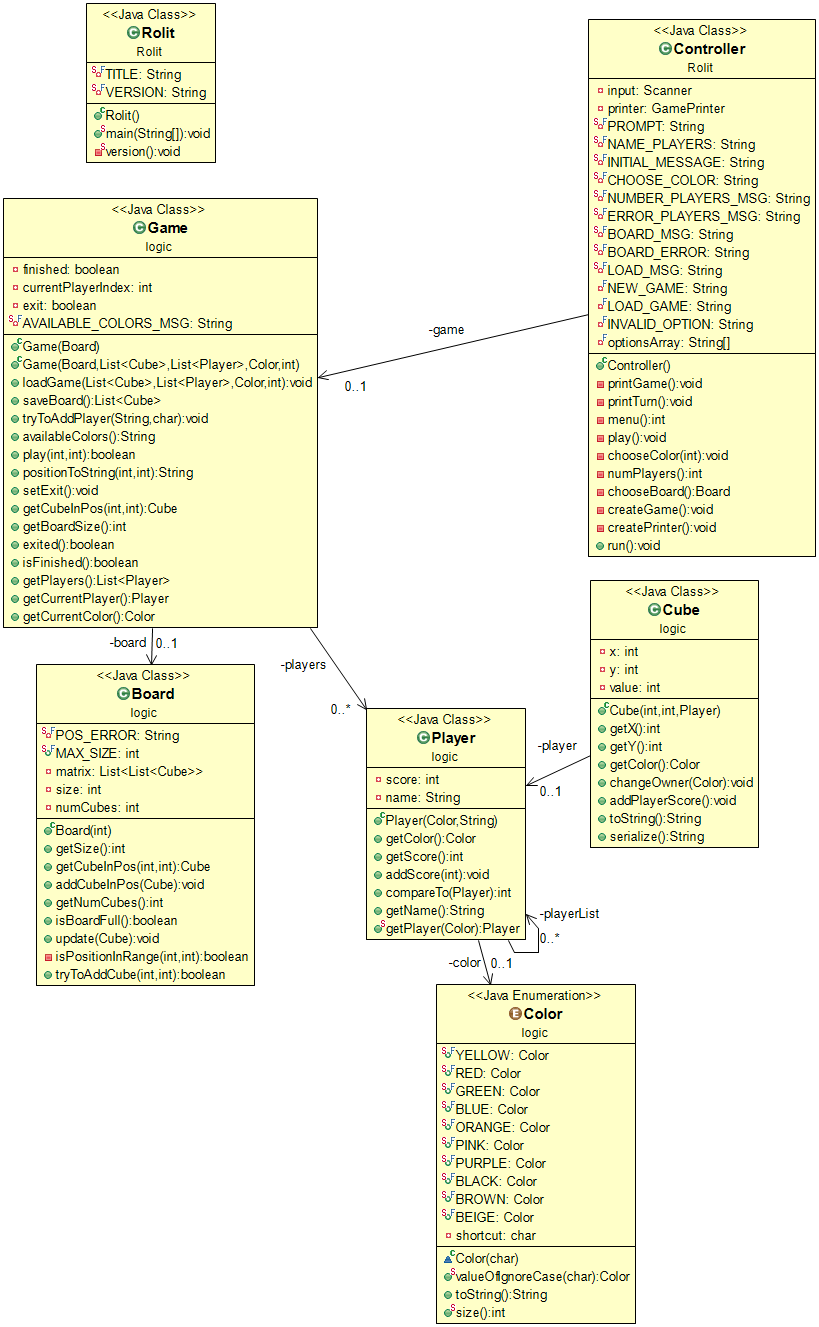
\includegraphics[scale=0.3]{diagramaclasesS2.png}
\end{center}

En esta segunda versión de Rolit, esta historia de usuario a penas sufre modificaciones, no obstante, la forma de implementarlas es algo distinta. Para poder apreciarlo mejor conviene comparar el diagrama de clases de este Sprint con el del Sprint anterior. Entre los cambios podemos destacar:
\begin{itemize}
\item \texttt{Game} ya no posee el mapa \texttt{Color}, \texttt{Player}.
\item \texttt{Player} tiene una lista de los \texttt{Player}.
\item \texttt{Cube} ya no tiene un atributo \texttt{Color}, ahora tiene un atributo \texttt{Player}
\item El tablero es un cuadrado de tamaño variable (entre 8 y 15), así como el número de jugadores también lo es (entre 2 y 10), por ello habrá 10 \texttt{Color} posibles. Para poder hacer un juego a gusto del cliente el \texttt{Controller} es el encargado de comunicarse con él, por medio de funciones como \texttt{ChooseColor()} o \texttt{ChooseBoard()}. 
\item Los cubos siguen siendo representados por letras significativas para cada \texttt{Color}.
\item el \texttt{main()} de \texttt{Rolit} tiene como única funcionalidad la creación del \texttt{Controller} y una llamada a su método \texttt{run()}.
\item Ahora el método \texttt{run()} es el encargado de crear el juego según desee el usuario y el bucle principal del juego estará en el método \texttt{play()}, un método nuevo que sería un intermediario entre \texttt{run()} de \texttt{Controller} y \texttt{play()} de Game, al que accedemos desde el \texttt{execute()} del comando \texttt{PlaceCube}.
\begin{center}
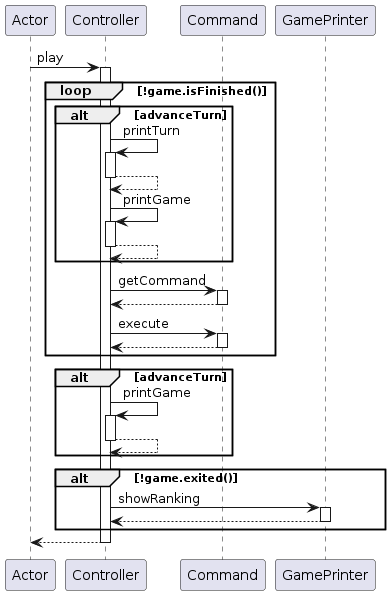
\includegraphics[scale=0.35]{playS2.png}
\end{center}
Como podemos apreciar en la imagen superior, ahora es \texttt{play()} el encargado de gestionar cuando termina el juego, así como de mostrar el ranking final del juego, que al igual que el anterior Sprint vendrá determinado por el \texttt{score} de los \texttt{Player}. Al añadir el comando \texttt{Exit} el bucle de \texttt{play()} de \texttt{Controller} podría terminar y que el juego no haya terminado, por eso es necesario hacer la comprobación al saltar de turno.

\item la función \texttt{play()}de \texttt{Game} es muy parecida a la del Sprint 1, no obstante, al pasar el método \texttt{update()} de la clase \texttt{Game} a la clase \texttt{Board} debemos actualizar el atributo \texttt{finished} y pasar de turno en el método \texttt{play()} de \texttt{Game}. 
\begin{center}
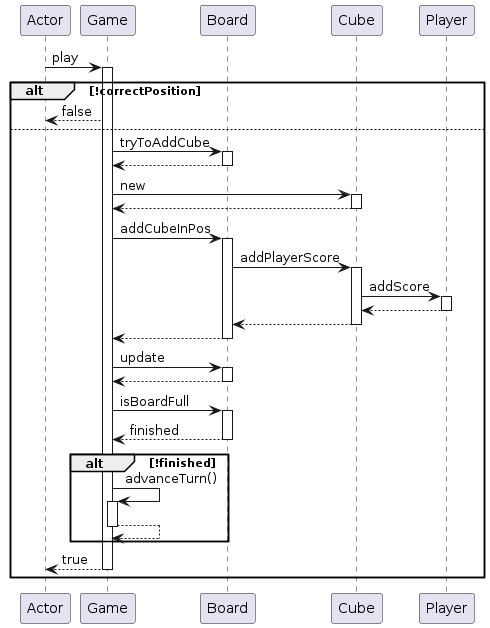
\includegraphics[scale=0.35]{playgameS2.png}
\end{center}

\item Tal y como se mencionó anteriormente el método \texttt{update()} pasó a estar en \texttt{Board} y en este caso su única funcionalidad es cambiar de color todos los cubos que quedan atrapados en las direcciones válidas. Esta será la versión final del método para todos los Sprints siguientes.
//TODO METERLE LA FOTO DEL DELGAU
\end{itemize} 
\end{sprint}

\begin{sprint}[3]

\begin{center}
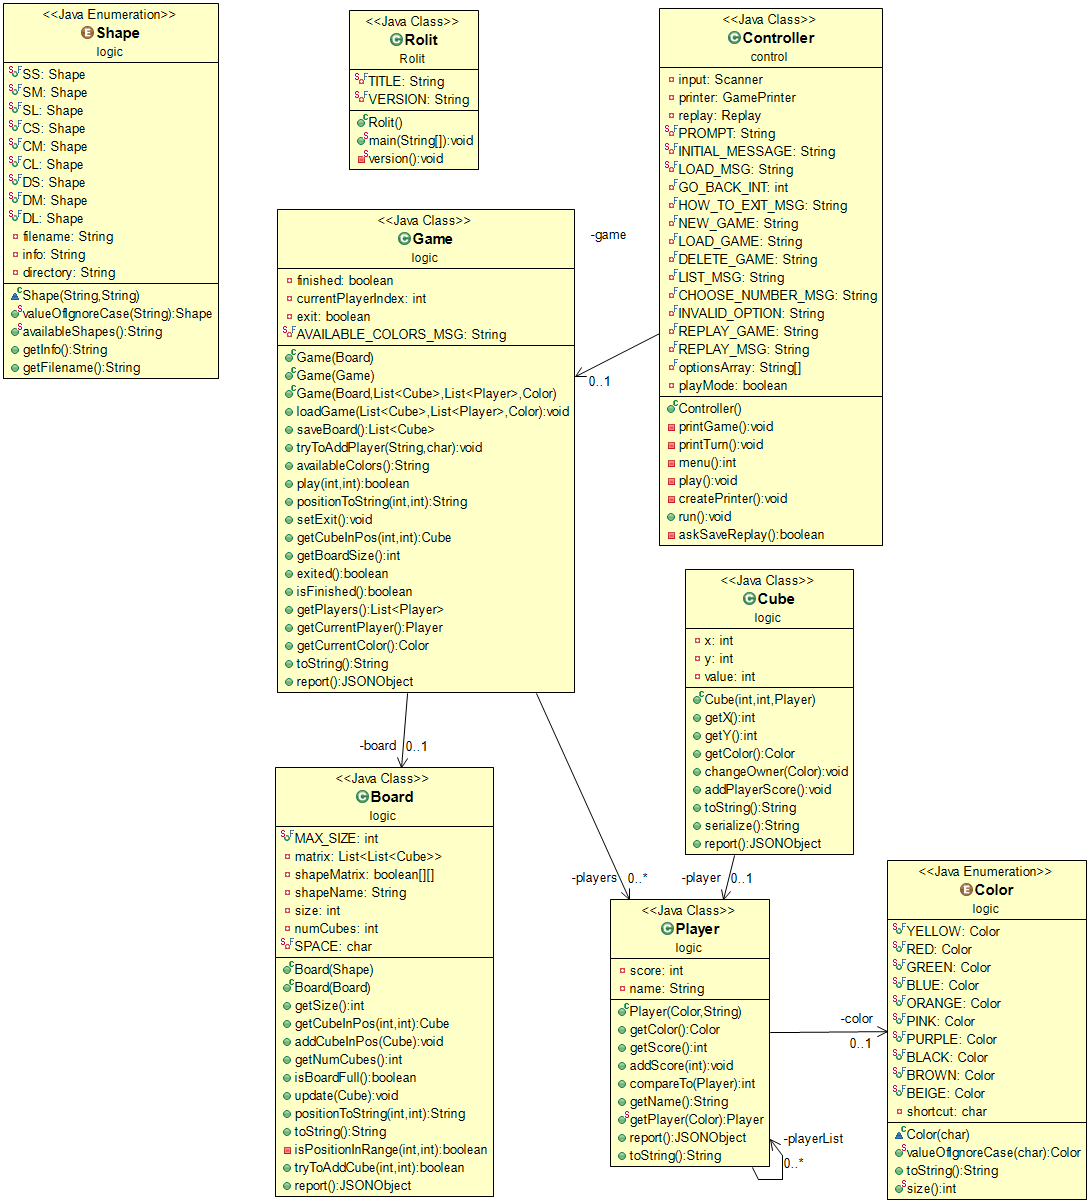
\includegraphics[scale=0.3]{diagramaclasesS3.png}
\end{center}

En esta tercera versión no hay apenas cambios, todo se gestiona de la misma manera salvo el \texttt{Board}. Ahora existen 9 tipos de tablero, hay tres formas y tres tamaños (grande, mediano, pequeño) para cada forma (rombo, círculo, cuadrado). Esto es posible gracias a métodos como \texttt{getShapeSize()} o \texttt{loadShape()} de la clase \texttt{SaveLoadManager}. 

\end{sprint}

\begin{sprint}[4]

A partir de este Sprint los cubos pasan a ser redondos y del \texttt{Color} que representan y se van introduciendo en las casillas del tablero.
\begin{center}
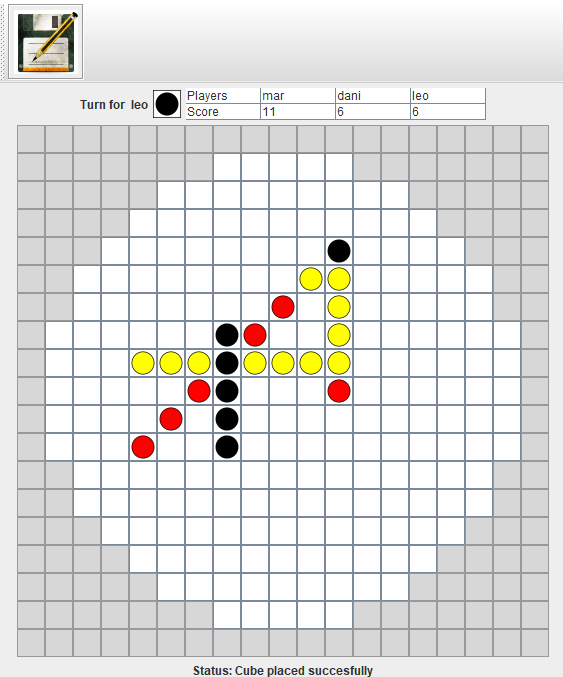
\includegraphics[scale=0.5]{cubos-redondos.png}
\end{center}

\end{sprint}

\subsection{Como usuario quiero poder jugar a Rolit con una interfaz agradable}

\subsubsection{JUANDI - Como usuario, me gustaría que se pudiesen personalizar los colores con los que jugamos cada jugador porque hace más visual el juego.}

\subsubsection{Como usuario, me gustaría que tenga una interfaz gráfica amable porque hace más fácil jugar.}
En este apartado, los primeros sprint realmente no son relevantes para comprender cuál ha sido la evolución del proyecto con respecto a esta historia de usuario, pues el desconocimiento de técnicas como el patrón del \textit{Modelo-Vista-Controlador} y la poca experiencia con proyectos grandes hace que el soporte gráfico y la encapsulación de la entrada salida en los primeros sprint sea realmente pobre una vez visto en persepctiva con el resultado final.

Sin embargo, poseen gran importancia los sprint 4 y 5, pues son en los que se incluye por primera vez una vista gráfica que no sea la de consola y porque por primera vez se formaliza una entrada salida controlada y a través de clases especializadas que son usadas a modo de componentes gráficos, pero para la consola.

\begin{sprint}[1]
Al comienzo del proyecto, el juego comenzaba (tras la generación de los objetos correspondientes) con la llamada al método \texttt{run()} del \texttt{Controller}. Este método contenía en su interior el propio menú en forma de sentencias de código:
\begin{lstlisting}
public void run() {

		System.out.println();
		System.out.println("Que desea?");
		System.out.println();
		for (int i = 0; i < arrayOpciones.length; ++i)
			System.out.println((i+1) + ". " + arrayOpciones[i]);
		
		int respuesta = 1;
		boolean repeat = true;
		...
\end{lstlisting}
y también la parte de impresión del tablero y de las jugadas conforme avanzaba el juego:
\begin{lstlisting}
while(!game.isFinished()) {
			String command;
			int posx, posy;
			boolean valido = false;
			
			printGame();
			
			while (!valido) {
				System.out.println(printer.showTurn());
				System.out.println("Introduce un comando:");
				System.out.println("c : Poner un cubo");
				System.out.println("s : Guardar partida");
				command = input.next();
				if ("c".equals(command)) {
					System.out.println("Introduce la posicion x: ");
					posx = input.nextInt();
					System.out.println("Introduce la posicion y: ");
					posy = input.nextInt();
					valido = game.play(posx, posy);
				}					
				else if("s".equals(command))
					saveLoadManager.saveGame();
				else
					System.out.println("Invalid Command");										
			}
			
		}
\end{lstlisting}
Tal y como se ve, principalmente la función más importante de impresión es la función \texttt{void printGame()} que se encargaba simplemente de hacer una llamada al método \texttt{String toString()} de la clase \texttt{GamePrinter} que era la experta en representación por pantalla de todo lo relativo al juego. Fundamentalmente, el desconocimiento del patrón Modelo-Vista-Controlador hizo que las instrucciones de uso del jugador o los diferentes menús de carga y guardado se hicieran en el propio método que se encargaba de hacer cada cosa, dificultando el poder hacer un diagrama de secuencia de cómo se imprime el menú o cómo se piden acciones.
\end{sprint}

\begin{sprint}[2]
En base a la experiencia en proyectos anteriores, durante este sprint se consolidó la clase \texttt{Controller} como la encargada de todos los procesos externos a los bucles del propio juego, es decir, se encargaba determinar el número de jugadores, el tipo de tablero, creación de los elementos del \texttt{Game}... Por tanto, el menú principal estaba en la clase \texttt{Controller}, concretamente la funcionalidad la encapsulaba la función \texttt{int menu()} que interactuaba con otros métodos privados de la clase para que el usuario pudiese decidir el resto de cosas y la funcionalidad de mostrar el juego seguía estando representada en la clase \texttt{GamePrinter} con el método \texttt{toString()}.

\begin{center}
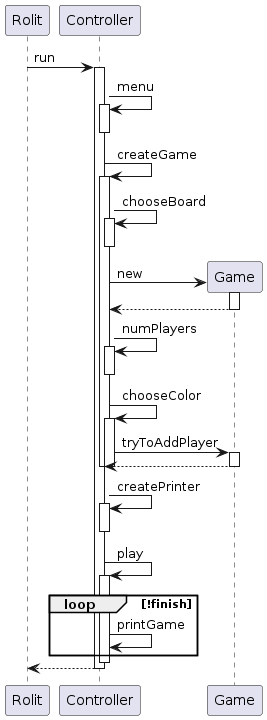
\includegraphics[scale=0.5]{MenuPpal_sprint2_seq}
\end{center}
\end{sprint}

Para formalizar esta primera aproximación a una encapsulación formal de cada una de las pantallas a métodos o clases concretas y especializadas, se generan las siguientes constantes en la clase \texttt{Controller} para tener unificados los mensajes que se envían:
\begin{lstlisting}
private static final String PROMPT = "Command > ";
	private static final String NAME_PLAYERS = "Name the players: ";
	private static final String INITIAL_MESSAGE = "Choose an option:";
	private static final String CHOOSE_COLOR = "Choose a color shortcut: ";
	private static final String NUMBER_PLAYERS_MSG = "Choose the number of players...";
	private static final String ERROR_PLAYERS_MSG = "Number of players must be...";
	private static final String BOARD_MSG = "Choose your board size [8 - "+ Board.MAX_SIZE + "]";
	private static final String BOARD_ERROR = "Board size must be a number between...";
	private static final String LOAD_MSG = "Type the name of the file (. to load default file): ";
\end{lstlisting}

\begin{sprint}[3]
El equipo de desarrollo observó que la clase \texttt{Controller} estaba perdiendo cohesión al asumir muchas responsabilidades que ciertamente no eran de un controlador. Para ello, se creó la clase \texttt{GameGenerator} como una antesala de lo que sería el patrón factoría. De este modo, el menú principal queda encapsulado en la función \texttt{int menu()} de la clase \texttt{Controller}, pero las pantallas donde se deciden el número de jugadores, el tipo de tablero, ... quedan como métodos privados de la nueva clase \texttt{GameGenerator} que es la encargada de saber crear el juego.
\begin{center}
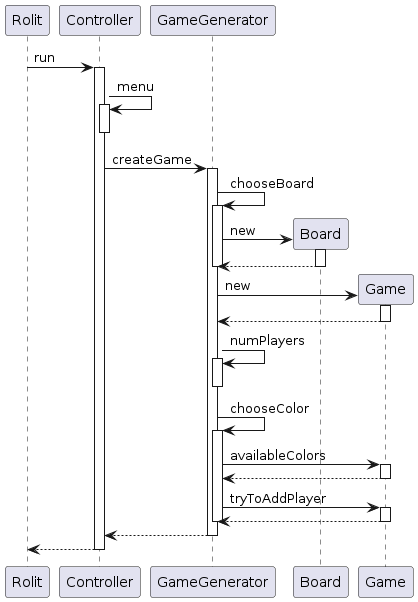
\includegraphics[scale=0.55]{MenuPpal_sprint3_seq}
\end{center}
En este caso, la función que imprime cada iteración del juego sigue siendo \texttt{printGame()} en \texttt{Controller} y aquellas que se encargan imprimir los mensajes de guardado y carga, así como de errores, siguen diseminadas por las respectivas clases que utilizan dichos métodos como sentencias \texttt{System.out.println("...")}, pues aún no se ha implementado el Modelo-Vista-Controllador.
\end{sprint}

\begin{sprint}[4]
\textbf{Console}

En este sprint, fundamentalmente se aplica el patrón Builder y Factorías a la situación del sprint anterior. En este caso, el menú principal sigue en el método \texttt{int menu()} de la clase \texttt{Controller} y los métodos que antes estaban en \texttt{GameGenerator} y se encargaban de pedir el número de jugadores, forma del tablero, ... por consola ahora forman parte del método \texttt{ask()} de las factorías (que por dentro saben que preguntar en cada caso).
\begin{center}
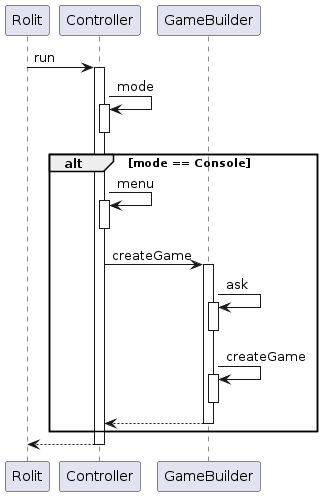
\includegraphics[scale=0.55]{MenuPpal_sprint4_seq}
\end{center}
A pesar de que se ha incluido el \textit{Modelo-Vista-Controlador} como patrón de arquitectura, la diferencia fundamental entre tener un nuevo hilo en \textit{Swing} y seguir en el mismo hilo que \textit{Main} ha hecho que no se haya formalizado una vista al uso para la parte de consola y que el código para ciertas excepciones y mensajes siga perdido por los lugares donde se producen dichas incidencias.

\textbf{GUI}

En este sprint se desarrolló una primera versión de la interfaz gráfica, lo cual involucra a un gran número de clases y métodos. Iniciemos un recorrido por cada uno de los componentes visuales explicando su finalidad

\underline{CeldaGUI}
\begin{center}

\includegraphics[scale=0.5]{yellowCube.png}

\includegraphics[scale=0.5]{emptyCell.png}
\end{center}

Esta clase representa cada una de las posiciones del tablero y puede ser vacía o tener un cubo. La mayor parte de funciones de esta clase  tienen como objetivo cambiar el color del cubo que representa cada celda.

\underline{BoardGUI}
\begin{center}
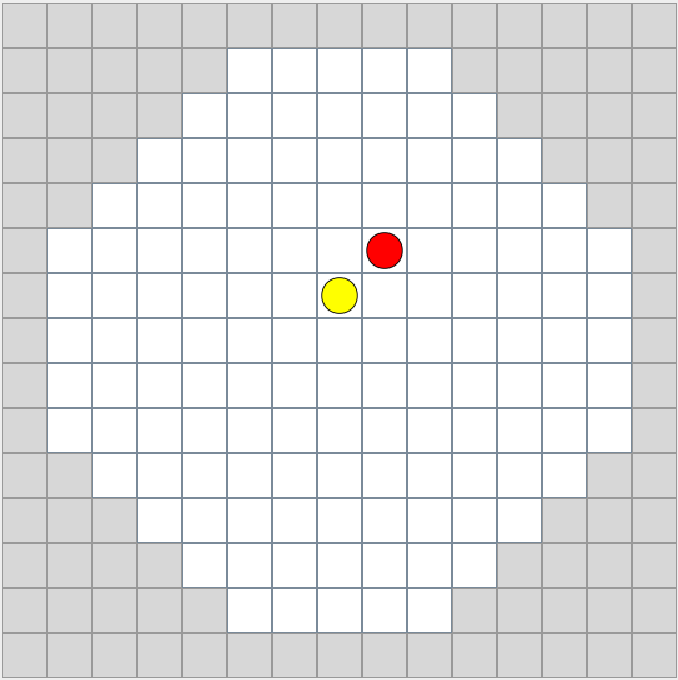
\includegraphics[scale=0.3]{board-gui-cubos-sprint3.png}
\end{center}

La clase \textit{BoardGUI} extiende de \textit{JPanel} y es la encargada de visualizar el tablero de la partida. Se puede apreciar que el tablero está formado por un conjunto de \textit{CeldaGUI}.

\underline{ControlPanel}
\begin{center}

\includegraphics[scale=0.8]{control-panel-sprint3.png}
\end{center}

El \textit{ControlPanel} es una \textit{JToolBar} que cuenta con un botón para guardar partidas, que puede ser pulsado en cualquier momento durante la ejecución del juego.

\begin{center}

\includegraphics[scale=0.8]{control-panel-replay-sprint3.png}
\end{center}

En el caso de las \textit{replays}, en el \textit{ControlPanel} aparecen dos flechas para poder recorrer los estados.

\underline{TurnAndRankingBar}
\begin{center}

\includegraphics[scale=1]{turn-ranking-panel-sprint3.png}
\end{center}

Esta clase es un \textit{JPanel} se encarga de mostrar a los usuarios del turno del jugador actual, las puntuaciones de cada uno de los participantes y la modalidad de juego.

\underline{StatusBar}


\underline{CreateGameDialog}
\begin{center}
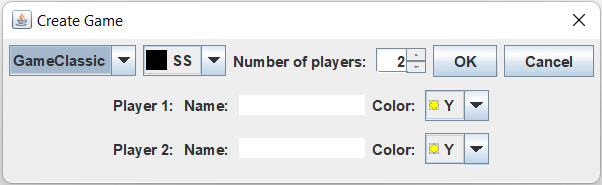
\includegraphics[scale=0.8]{create-game-sprint3.png}
\end{center}

Como su propio nombre indica, esta ventana extiende de \textit{JDialog} y tiene como objetivo poder configurar una partida desde cero, combinando todas las características posibles para crear un juego a gusto de los usuarios.

En esta pantalla el usuario elige el modo de juego para la partida (\textit{GameClassic} o \textit{GameTeams}), la forma y tamaño del tablero (cuadrado, círculo o rombo, pequeño, mediano o grande), el número de jugadores (entre 2 y 10, ambos inclusive) y el nombre y color de cada jugador.

En caso de seleccionarse el modo por equipos, el usuario introducirá el nombre de ambos equipos y el equipo al que pertenece cada jugador.

Una vez el usuario presiona el botón \textit{OK} se le lleva a la pantalla de juego.

Si el usuario presiona \textit{Cancel} se le lleva de vuelta a la pantalla principal.

\underline{LoadGameDialog}
\begin{center}
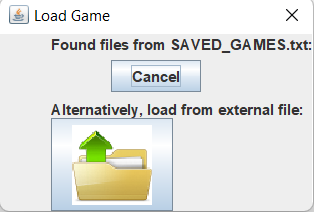
\includegraphics[scale=0.8]{load-dialog-sprint3.png}
\end{center}

En esta pantalla se muestra una lista con las partidas guardadas, de forma que si se elige una de estas partidas se cargará inmediatamente.

Aparece también debajo un botón de carga de ficheros que abre un  \textit{JFileChooser} por si se quiere cargar un juego que no esté incluido en la lista de partidas guardadas.

\underline{DeleteGameDialog}
\begin{center}
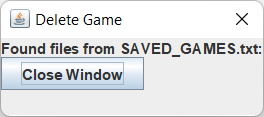
\includegraphics[scale=0.8]{delete-dialog-sprint3.png}
\end{center}

En esta pantalla se muestra la lista de partidas guardadas y un botón para confirmar el borrado. Con esto, si se selecciona una de las partidas guardadas y se presiona el botón inferior, la lista se elimina de la lista de partidas guardadas.

\underline{StatusBar}
\begin{center}

\includegraphics[scale=0.8]{status-bar-sprint3.png}
\end{center}

La \textit{StatusBar} es un \textit{JPanel} que se encarga de mostrar información relevante durante la partida, como mensajes de error o de confimación, otorgándole al usuario un feedback adecuado.

\underline{MainWindow}
\begin{center}
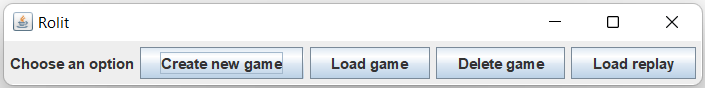
\includegraphics[scale=0.8]{menu-sprint3.png}
\end{center}

Inicialmente la ventana principal comienza con una pantalla en la que se muestran cuatro opciones a elegir por el usuario: \textit{Create new game, Load game, Delete game, Load replay}.

Si se ha decidido jugar a una partida o cargar una replay, el panel principal de la \textit{MainWindow} será reemplazado por un panel que contiene, de arriba a abajo, un ControlPanel, una TurnAndRankingBar, un BoardGUI y una StatusBar.

\begin{center}
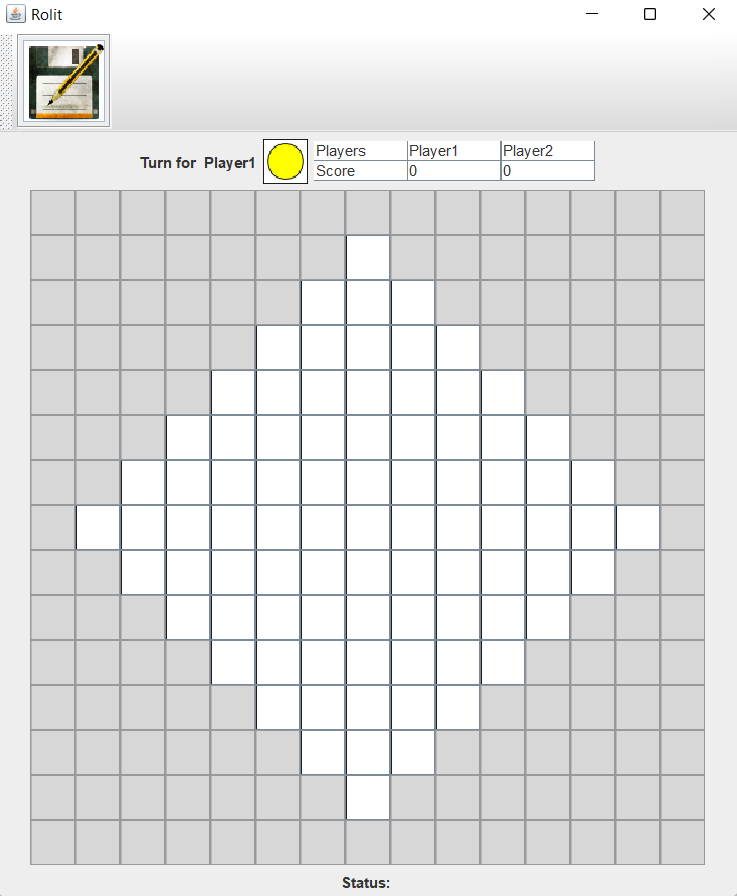
\includegraphics[scale=0.9]{game-sprint3.png}
%FIXME CENTRAR
Jugar una partida
\end{center}

\begin{center}
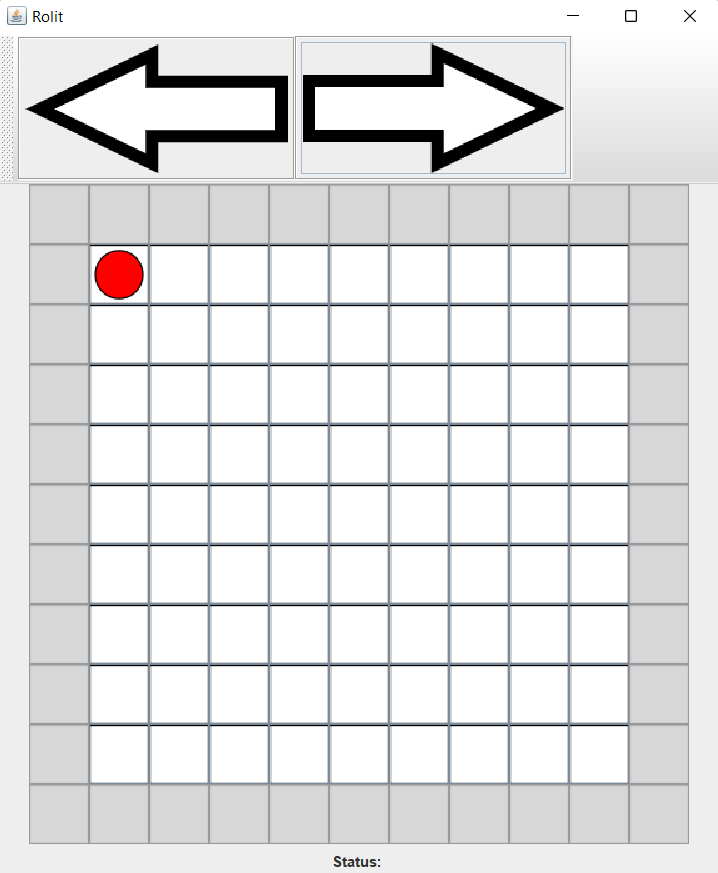
\includegraphics[scale=0.9]{replay-sprint3.png}
%FIXME CENTRAR
Reproducir una \textit{replay}
\end{center}

\underline{Funcionamiento interno}

Una vez visualizadas todas las pantallas es el momento de hablar su funcionamiento interno. Al introducir la GUI decidimos aplicar el patrón MVC, de manera que los futuros cambios en el modelo produzcan modificaciones mínimas en la vista y controlador y viceversa. Para más información sobre el Modelo-Vista-Controlador puede hacer click aquí. %FIXME AÑADIR REFERENCIA AL MVC

Para la comunicación de las vistas con los modelos se decidió utilizar el patrón observador, así son los propios modelos los que comunican a las vistas cuando deben actualizarse.

La implementación de este patrón se llevó a cabo mediante tres interfaces: Observable, diseñada para los modelos; RolitObserver, pensada para los observadores de la clase \textit{Game}; y ReplayObserver, que utilizan los observadores de la clase \textit{Replay}.

\begin{center}
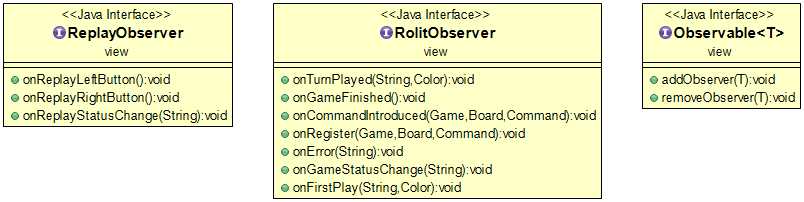
\includegraphics[scale=0.43]{observadores-sprint4.png}
\end{center}

En el caso de la GUI, la comunicación con los modelos se lleva a cabo a través de los \textit{ActionListeners} de los botones, que ejecutan el comando que corresponda.

\end{sprint}

\begin{sprint}[5]
\textbf{Console}

En el sprint 5, la evidencia de las limitaciones que tiene tener la consola tan poco definida en comparación con la programación de componentes de \textit{Swing} y la implementación de un hilo a parte para el modelo hacen posible que se cree una serie de clases a modo de ``componentes'' para formalizar de una vez la vista del modo consola:
\begin{center}
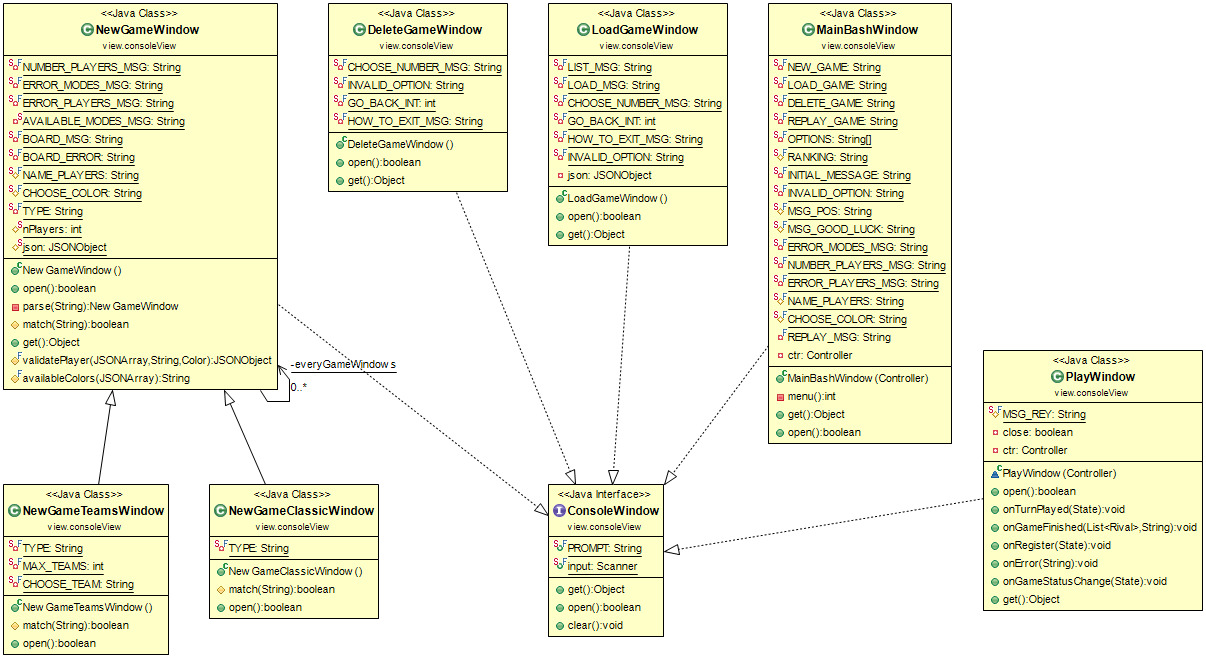
\includegraphics[scale=0.55, angle=90]{DiagramaClasesConsola}
\end{center}
Tal y como se ve en el diagrama de clases, hemos creado una interfaz \texttt{ConsoleWindow} que será la abstracción que represente un ``componente de la consola''. Todas las posibles ventanas del juego extenderán de dicha interfaz y el método \texttt{bool open()} será el que indicará que el componente se muestra y empieza a funcionar. Además, cabe destacar que hacerlo de esta manera permite que las clases que representan a las ventanas en la consola ahora puedan ser observadores, por lo que cubrimos mucho mejor el \textit{MVC} y además nos permite simplificar el comportamiento del modelo al ser unificado para cualquier vista la forma de notificar los cambios.

Con todo esto conseguimos que al iniciar el juego en la clase \texttt{Rolit} y seleccionar el modo de vista deseado, se escoja qué componente (la \texttt{MainWindow} de \textit{Swing} o la \texttt{MainBashWindow} de la consola) se abrirá para empezar la vista. Esto permite que a nivel de vistas solo trabajemos con abstracciones de las clases que conforman cada ventana, por tanto, agregar nuevas ventanas en la consola se reduce a crear una nueva clase que encapsule lo que se espera de la nueva ventana. De este modo, el menú principal de elección sobre un nuevo juego, cargar uno antiguo, etc. queda como:
\begin{center}
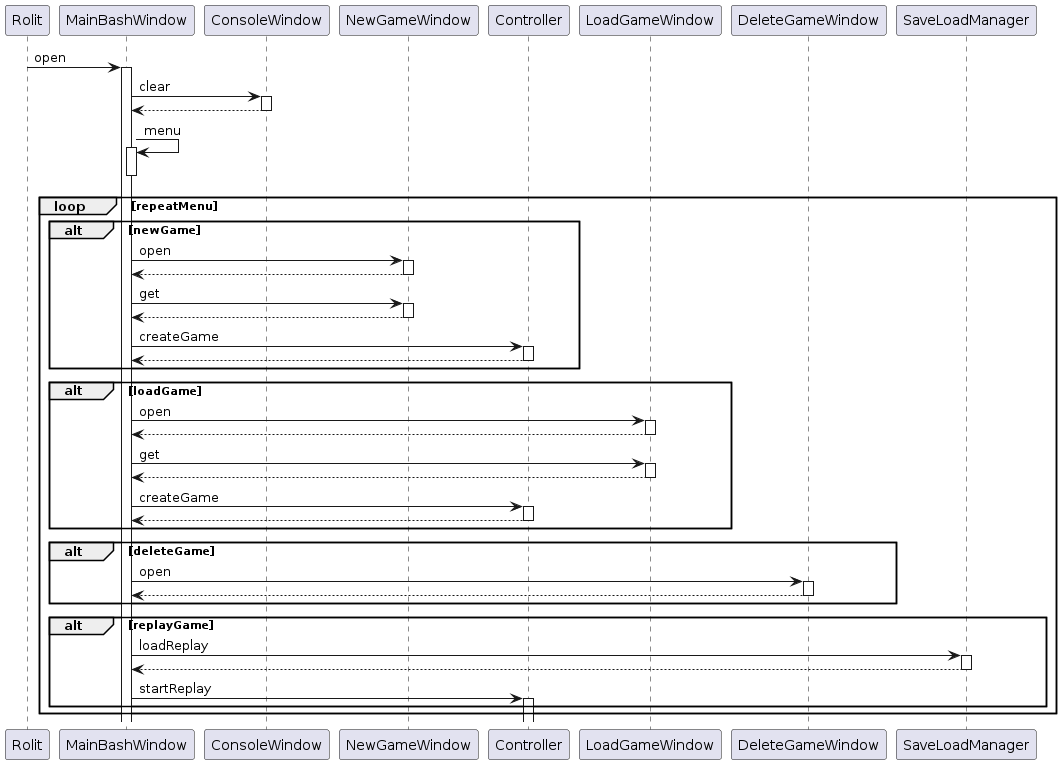
\includegraphics[scale=0.40]{MenuPpal_sprint5_seq}
\end{center}
Y el funcionamiento interno de cada una de las ventanas puede verse de la siguiente manera:
\begin{itemize}
\item \underline{NewGameWindow}: está implementada utilizando el patrón factoría (puesto que son clases íntimamente ligadas a los \texttt{Builder} ya que son las ventanas donde se crea el juego) y heredan la funcionalidad que tenían los métodos \texttt{void ask()} de los \texttt{Builder}.
\begin{center}
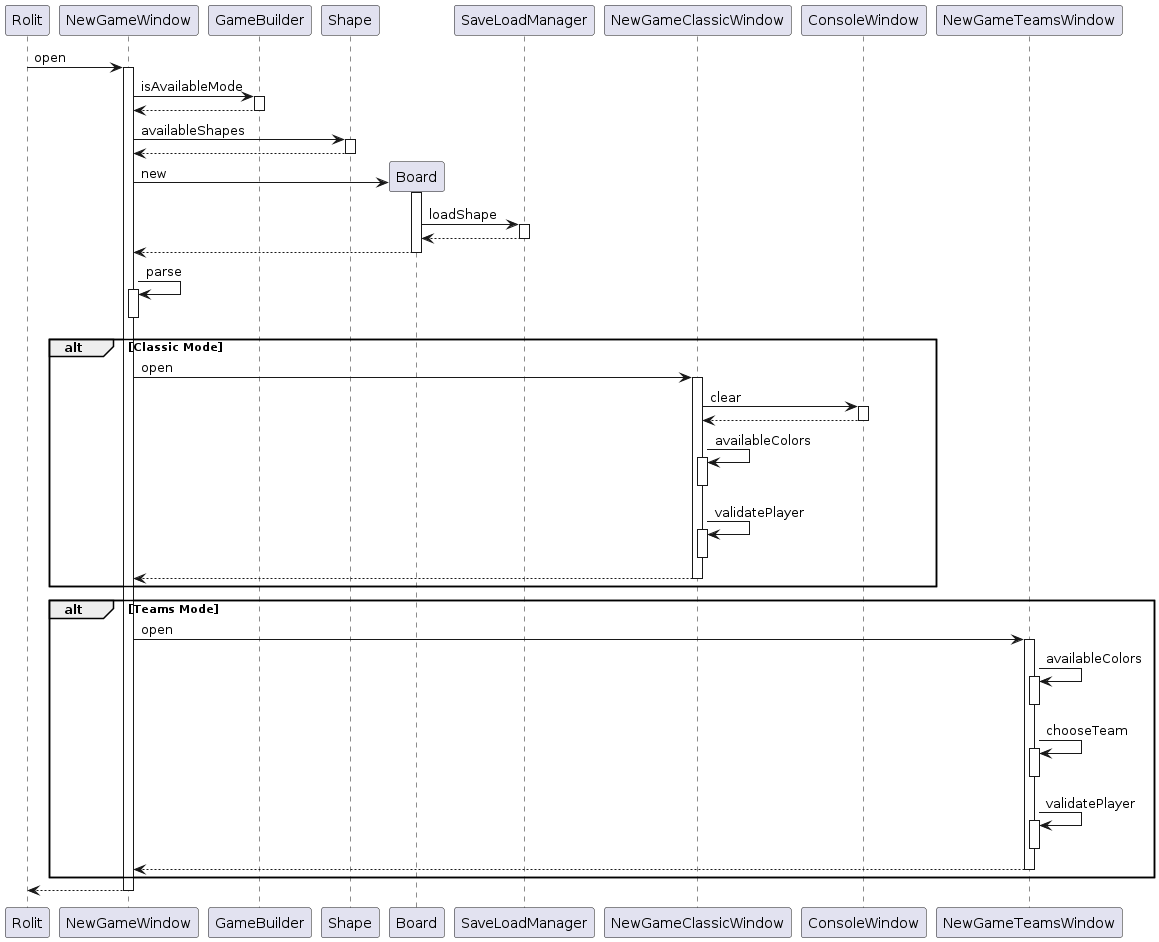
\includegraphics[scale=0.40, angle=90]{NewGameWindow_sprint5_seq}
\end{center}

\item \underline{LoadGameWindow}: es una clase de ventana que principalmente hace las llamadas adecuadas a \texttt{SaveLoadManager} que el la clase \textit{Experta} en el manejo de flujo de ficheros de carga y guardado.
\begin{center}
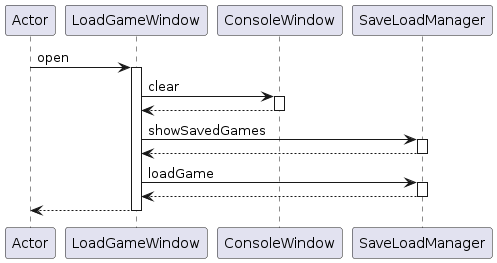
\includegraphics[scale=0.5]{LoadGameWindow_sprint5_seq}
\end{center}

\item \underline{DeleteGameWindow}: es una clase de ventana que de nuevo se encarga de gestionar las llamadas correspondientes a \texttt{SaveLoadManager} para borrar uno de los juegos cargados.
\begin{center}
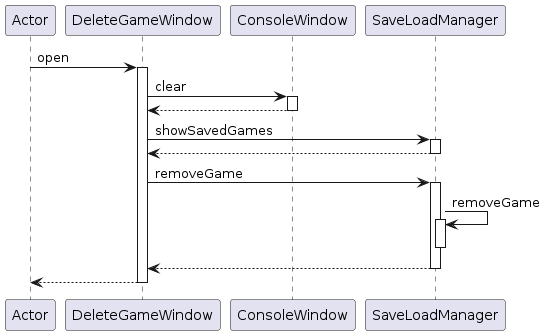
\includegraphics[scale=0.5]{DeleteGameWindow_sprint5_seq}
\end{center}
\end{itemize}

La clase que principalmente soporta la ventana de consola una vez se va a comenzar a jugar es la clase \texttt{PlayWindow} que se mantiene abierta hasta que el juego notifique que ha terminado. En dicha ventana se generan a través de la entrada por teclado, los comandos que posteriormente cambiarán el estado del modelo y está implementada de forma que sea un observador, tanto para percibir los cambios que ocurren este y mostrarlos adecuadamente como para reaccionar en consecuencia mostrando cosas según el tipo de juego que tengamos (aunque ella solo maneja la abstracción de un \texttt{Game} cualquiera):
\begin{center}
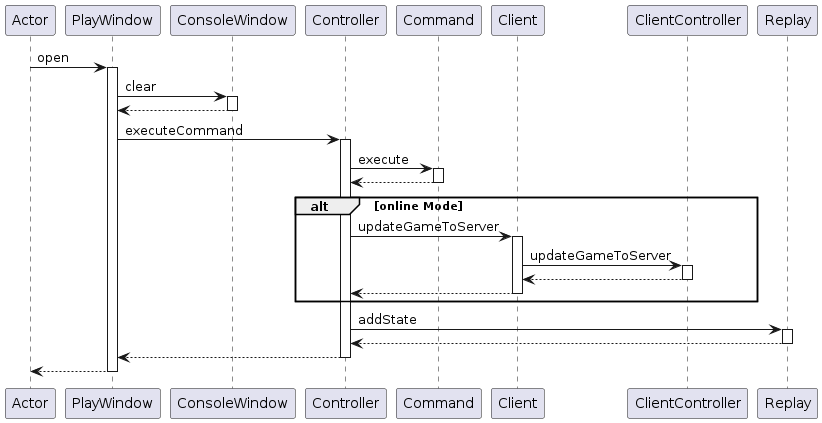
\includegraphics[scale=0.5]{PlayWindow_sprint5_seq}
\end{center}

\textbf{GUI}

\underline{MainWindow}

La incorporación de la funcionalidad para jugar en red trajo consigo  la necesidad de añadir nuevos botones al menú principal para poder acceder a ella.

\begin{center}
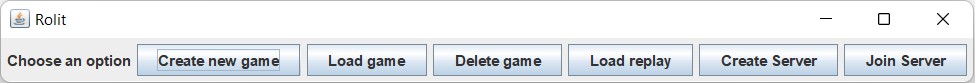
\includegraphics[scale=0.6]{menu-sprint5.png}
\end{center}

\underline{CreateGameDialog}

\begin{center}
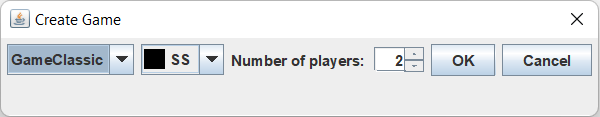
\includegraphics[scale=0.8]{create-game-sprint5.png}
\end{center}

Al configurar la partida de un servidor no es posible introducir la información de los jugadores, pues es cada uno individualmente quien decide su nombre y color desde su ordenador.

Por este motivo, se añadió un atributo al constructor de \textit{CreateGameDialog} que permite ocultar el panel que contiene los componentes para introducir los datos de los jugadores.

\underline{CreateServerDialog}
\begin{center}
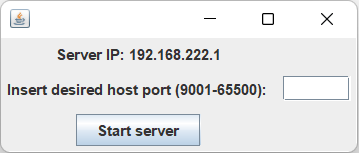
\includegraphics[scale=0.8]{create-server-sprint5.png}
\end{center}

Para poder crear el servidor el usuario debe elegir en qué puerto hostearlo, para ello se creó este \textit{JDialog}, que abre el servidor una vez se pulsa el botón ``Start Server".

En esta versión del juego, la poca experiencia con el manejo de hilos del equipo de desarrollo provocó que esta ventana se quedase pillada hasta que todos los participantes se unieran al servidor.

\underline{JoinServerDialog}
\begin{center}
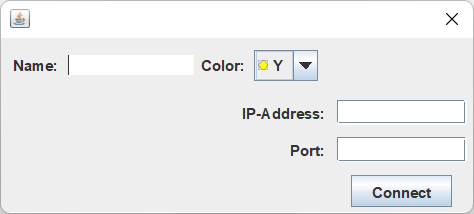
\includegraphics[scale=0.8]{join-server-sprint5.png}
\end{center}

Como ya se ha mencionado anteriormente, es cada usuario al unirse al servidor quien decide su nombre y su color. La clase \textit{JoinServerDialog} es la encargada de ello, además de recoger la IP y el puerto del servidor al que se quiere acceder.

\underline{Funcionamiento interno}

En el sprint anterior nuestra única intención era hacer una interfaz gráfica funcional, y ese objetivo fue alcanzado exitosamente. Sin embargo, la GUI accedía directamente a todos los métodos que necesitase de la clase \textit{Game}, algo que no es correcto desde el punto de vista de la programación orientada objetos.

Para solventar este problema planteamos inicialmente el uso de objetos transferencia que restringiesen los métodos de las clases que eran necesarias para visualizar el juego.

Finalmente, esta idea fue rechazada en favor de reutilizar el código ya existente. Así, se decidió que la información se transmitiese mediante la clase \textit{State} creada originalmente para reproducir las \textit{replays}, pues al fin y al cabo, un estado representa una serialización del juego y contiene toda la información necesaria.

\begin{center}
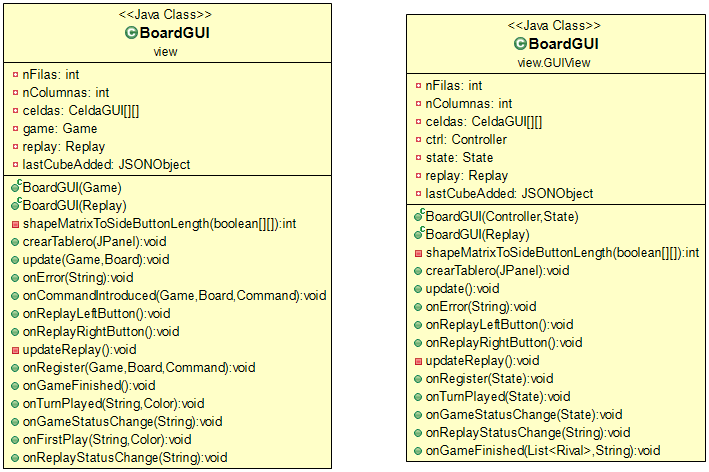
\includegraphics[scale=0.5]{board-gui-evol.png}

Evolución de la clase \textit{BoardGUI}. Sprint 4 (izq) y Sprint 5 (der)
\end{center}

Por consiguiente, todas las instancias de clases relacionadas con el modelo de \textit{Game} fueron eliminadas y reemplazadas por estados y JSONObjects. Para ello fue necesario añadir nuevos métodos a la clase \textit{State}.

\begin{center}
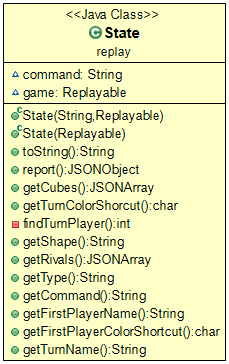
\includegraphics[scale=0.5]{state-sprint5.png}
\end{center}

\end{sprint}

\begin{sprint}[6]
\textbf{Console}

Los componentes a modo de ventanas de la consola no sufrieron más cambios más allá del sprint 5, únicamente se corrigieron errores en los \texttt{input.nextLine()} de la lectura puesto que fallaba al no consumir saltos de línea abandonados en el buffer.

\textbf{GUI}

En este sprint la GUI fue refactorizada por completo, cambiando tanto visualmente, como a nivel de funcionamiento interno en algunas clases para hacer el código más manejable.

\underline{Creación de RolitComponents}

Hasta este momento el proyecto utilizada los componentes visuales de Java poder defecto, dando lugar a una interfaz gráfica funcional, pero con carencias visuales.

Para el estilo de los componentes, se optó por una interfaz minimalista basada en el color blanco y en el azul que aparece en el logo del juego Rolit, al que se denominó \textit{BLUE\_ROLIT}.

Los \textit{RolitComponents}, como la clase \textit{RolitButton} o \textit{RolitTextArea}, además de homogeneizar el entorno visual facilitan los cambios de estilo en un futuro.

Veamos el resultado gráfico tras la aplicación de estos componentes, sumado a re-estructuraciones en los Layouts y la inclusión de nuevas imágenes e iconos

\underline{MainWindow}
\begin{center}
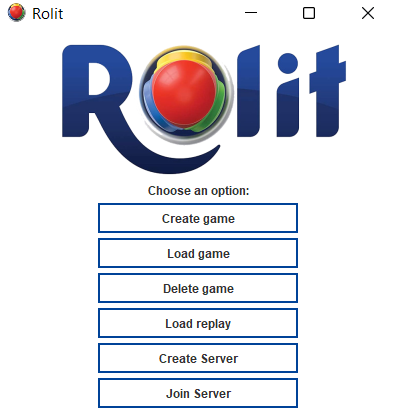
\includegraphics[scale=1]{menu-sprint-6.png}

\end{center}

\begin{center}
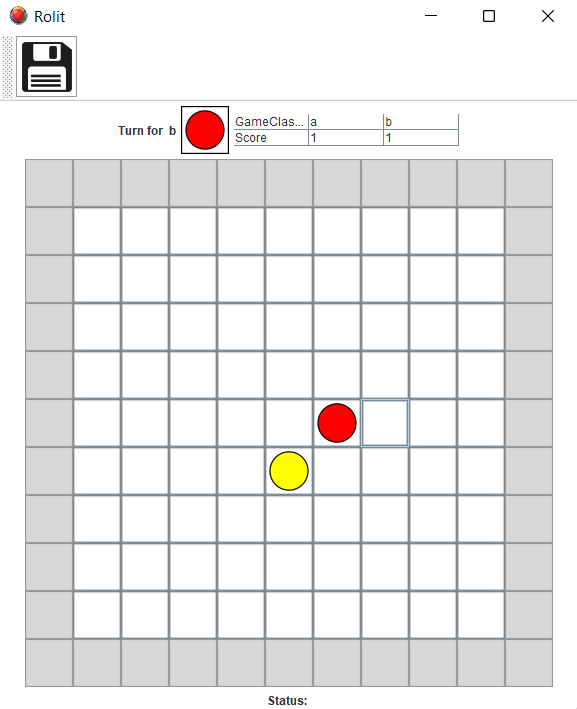
\includegraphics[scale=1]{partida-sprint-6.png}

Jugar una partida
\end{center}

\begin{center}
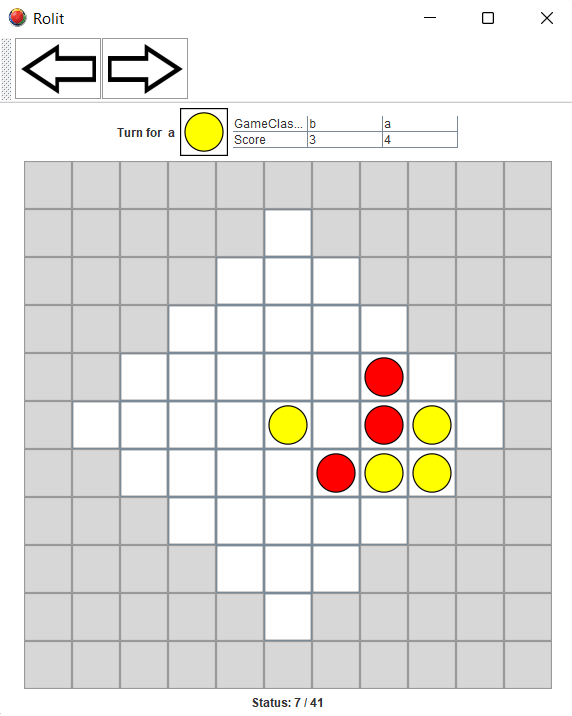
\includegraphics[scale=1]{replay-sprint-6.png}

Reproducir una \textit{replay}
\end{center}

\underline{CreateGame package}

En sprints anteriores había una clase encargada de crear y gestionar todos los componentes visuales necesarios para crear un juego nuevo, resultando en una clase demasiado compleja.

Por ello, la antigua clase \textit{CreateGameDialog}, fue dividida en otras más pequeñas. Dando lugar a:

\begin{itemize}
\item \textit{PlayerDataPanel}: panel que contiene los componentes necesarios para obtener la información de un jugador.
\begin{center}

\includegraphics[scale=1]{player-data-panel.png}
\end{center}
\item \textit{TeamDataPanel}: panel que contiene los componentes necesarios para obtener la información de un equipo.
\begin{center}

\includegraphics[scale=1]{team-data-panel.png}
\end{center}
\item \textit{CreatePlayersPanel}: conjunto de \textit{PlayerDataPanel}.
\item \textit{CreateTeamsPanel}: conjunto de \textit{TeamDataPanel}.
\item \textit{GameConfigurationPanel}: panel encargado de obtener la configuración básica del juego: modo de juego, forma, numero de jugadores...
\begin{center}
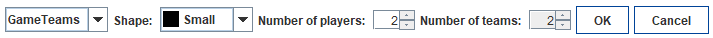
\includegraphics[scale=0.75]{game-config-panel.png}
\end{center}
\item \textit{CreateGameDialog}: ventana de diálogo que contiene un \textit{GameConfigurationPanel} y un \textit{CreateTeamsPanel}.
\begin{center}
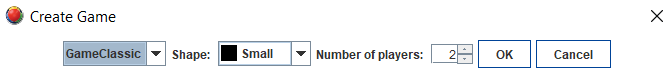
\includegraphics[scale=0.8]{create-game-sprint6.png}
\end{center}
\item \textit{CreateGameWithPlayersDialog}: extiende a \textit{CreateGameDialog}, añadiendo un \textit{CreatePlayersPanel}.
\begin{center}
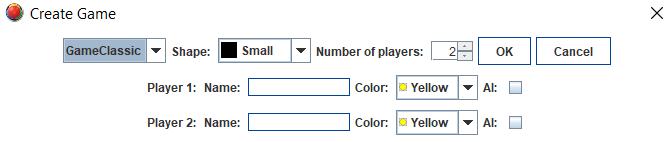
\includegraphics[scale=0.75]{create-game-players-sprint6.png}
\end{center}
\end{itemize}


\underline{LoadFileDialog}
\begin{center}
\includegraphics[scale=1]{load-game-sprint-6.png}
\end{center}

Las clases \textit{LoadGameDialog} y \textit{LoadReplayDialog} fueron abstraidas en \textit{LoadFileDialog}, que permite cargar tanto partidas como \textit{replays}, dependiendo del botón que se pulse.

\underline{DeleteGameDialog}
\begin{center}
\includegraphics[scale=1]{delete-dialog-sprint6.png}
\end{center}

\underline{CreateServerDialog}

\begin{center}
\includegraphics[scale=1]{server-setup-sprint-6.png}
\end{center}

Además, una vez creado el servidor, el usuario que está hosteandolo recibe feedback de cuanta gente se ha unido.

\begin{center}
\includegraphics[scale=1]{server-feedback.png}
\end{center}


\end{sprint}

\underline{JoinServerDialog}
\begin{center}
\includegraphics[scale=1]{join-server-sprint-6.png}
\end{center}

Los usuarios también reciben feedback del servidor, mostrándose una venta que les invita a esperar a los demás.

\begin{center}
\includegraphics[scale=0.85]{user-feedback.png}
\end{center}

\underline{Ranking}

Además, en este sprint se incluyó en la GUI un ranking final donde se muestran los tres primeros puestos. En caso de que solo haya dos jugadores solo se mostrarán esos dos.

\begin{center}
\includegraphics[scale=0.85]{ranking-2players.png}

Ranking para dos jugadores
\end{center}

\begin{center}
\includegraphics[scale=0.85]{ranking-3players.png}

Ranking para más de dos jugadores
\end{center}

\newpage

\subsection{Como usuario quiero que Rolit introduzca características innovadoras pensando en las posibilidades que brinda el multijugador}

\subsubsection{Como usuario, me gustaría que se pudiera jugar contra una inteligencia artificial, así como que ellas jugaran solas}
\begin{sprint}[5]
Este fue el Sprint en el que se empezaron a desarrollar las distintas estrategias de las inteligencias artificiales. Se planearon tres, recogidas en las siguiente clases, todas herederas de la clase abstracta Strategy: RandomStrategy, GreedyStrategy y MinimaxStrategy.

La idea de la estrategia es que, cuando le toque jugar a una inteligencia artificial, la estrategia se encarge de calcular su siguiente movimiento y este se ejecutase inmediatamente después de su cálculo.

Para hacer esto, hemos hecho uso del \textbf{patrón estrategia}. Este patrón permite mantener un conjunto de algoritmos para la resolución de una tarea de distintas formas, de forma que se pueda dinámicamente elegir un algoritmo u otro en tiempo de ejecución. La explicación de como se ha llevado a cabo el patrón se explica a continuación.

Para encapsular está lógica se creo la clase abstracta Strategy, para que cada estrategia en particular fuera una clase heredera de esta.

Se han desarrollado tres estrategias, que suponen tres niveles de dificultad distintos, y la lógica de estas está recogida en las siguientes clases: RandomStrategy, GreedyStrategy y MinimaxStrategy.

\textbf{RandomStrategy}:
La idea es que se genere una posición cualquiera en el tablero, siempre y cuando esta sea válida. Esta es la posición que la inteligencia artificial jugará.
Lógicamente, la tendencia general las inteligencias artificiales que aplican esta estrategia es no obtener una gran cantidad de puntos, por lo que esta estrategia es la de nivel fácil.

\textbf{GreedyStrategy}:
Esta estrategia tiene por intención analizar el tablero en busca de la posición que le garantiza al jugador el máximo número de puntos en este mismo turno. Esta estrategia lleva a jugadas mucho mejores y elaboradas, pero sigue sin ser la mejor, así que representa el nivel de dificultad medio.

\textbf{MinimaxStrategy}:
Esta estrategia realiza el cálculo de la posición en la que jugar el siguiente turno a través de una adaptación a Rolit del algoritmo Minimax. Este algoritmo se explica en el \hyperref[ch:AnexoIII]{Anexo III}. Este es un algoritmo con un nivel de sofisticación considerablemente mayor que los de las anteriores estrategias y por ello (y tras comprobación en base a la simulación de numerosas partidas) este algoritmo representa el nivel de dificultad alto. Se dan más detalles de la implementación en la subsección  \hyperref[subsubsec:MinimaxStrategy]{MinimaxStrategy}.

Para hacer el cómputo de todas las simulaciones, usar como representación la que nos proporciona la clase \texttt{Board} resulta inviable, por lo que se ha creado una nueva clase a modo de representación puramente funcional del tablero orientada a las simulaciones, llamada \texttt{SimplifiedBoard}.

Se pueden ver detalles de la implementación de estas clases en la subsección \hyperref[subsec:Strategy]{Strategy}.

El cómputo del movimiento a jugar a través de la estrategia Minimax, llevado a cabo en el método calculateNextMove(), se ilustra en el siguiente diagrama:

\begin{center}
\centering
\includegraphics[scale=0.45]{MinimaxStrategy.calculateNextMove()-sprint5.png}
\end{center}

\end{sprint}

\begin{sprint}[6]
Por motivos de eficiencia de los cálculos de \texttt{MinimaxStrategy}, se ha implementado de forma complementaria la poda Alfa-Beta. Los detalles acerca de este concepto se explican en el \hyperref[ch:AnexoIII]{Anexo III}.

Esta poda ha sido muy útil para reducir costes de cálculo, y el nuevo algoritmo mejorado queda reflejado en el siguiente diagrama:

\begin{center}
\centering
\includegraphics[scale=0.5]{MinimaxStrategy.calculateNextMove()-sprint6.png}
\end{center}

\end{sprint}

\newpage

\subsubsection{Como usuario, me gustaría que se pudiera jugar en red.}
\begin{sprint}[5]
En cuanto a la tarea de añadir un modo de juego en red, se concibe, planea e implementa la funcionalidad de red casi por completo, consigue llegar a una versión funcional de juego en red en GameClassic.

En cuanto al servidor, se define y se mantiene en todos los sprints la característica de que el servidor no posee el modelo, si no que es un intemediario entre clientes (pasando información procedente de un cliente al resto de clientes, para que estos últimos actualicen sus modelos). El diálogo ServerView interactúa con el servidor a la hora de dejar al usuario especificar los detalles sobre los que el servidor operará (puerto).

En cuanto al cliente, se define y se mantiene en todos los sprints la característica de que el cliente es el que posee el modelo, Cada vez que se hace una modificación en el modelo del cliente, se envía al servidor la información del juego; el servidor procede a actualizar la información del modelo del resto de clientes conectados.

Al final del Sprint, los objetivos alcanzados son los siguientes:

\begin{itemize}
\item Determinar si el servidor, o por el contrario el cliente, debería poseer el modelo. Optamos por la segunda opción.

\item Definir toda la estructura en cuanto a relaciones jerárquicas de clases y dependencias entre las mismas.

\item Crear un número suficiente de diálogos en GUI que permitan la conexión en red. Entre ellos, se encuentran:
\begin{itemize}
\item ServerView
\item JoinServerDialog
\end{itemize}

El diseño y evolución pormenorizados de estos diálogos se encuentran en el apartado de la historia de usuario dedicada a la interfaz.

\item Reutilizamiento del código del diálogo de crear partida, adaptado a las circunstancias de red.

\item Poder jugar a una partida GameClassic en red de forma satisfactoria.

\end{itemize}

Aun así, otros de los objetivos propuestos no son implementados por falta de tiempo y de dependencia con otras de las partes del desarrollo no concluidos. Estos objetivos son:

\begin{itemize}
\item Crear más diálogos que aporten feedback para la conexión, tanto de la perspectiva del cliente como del servidor.

\item Llegar a una versión completamente refactorizada y con métodos simplificados.

\item Implementar el juego en red en GameTeams.
\end{itemize}

Presentamos los diagramas UML de este Sprint.

El UML de clases es el siguiente:

\begin{center}
\includegraphics[scale=0.45]{UMLClasesRedSprint5.png} 
\end{center}

Presentamos los diagramas de secuencia de este Sprint.

\begin{itemize}

\item Cómo se realizan las conexiones

\begin{center}
\includegraphics[scale=0.45]{umlconexiones.png} 
\end{center}

\item Cómo se inicia una partida

\begin{center}
\includegraphics[scale=0.45]{empezarPartidaUml.png} 
\end{center}

\item Cómo se envía y recibe una jugada

\begin{center}
\includegraphics[scale=0.45]{juegoTipicoUml.png} 
\end{center}

\end{itemize}

\end{sprint}



\begin{sprint}[6]
En cuanto a la red, se alcanzan los objetivos propuestos que quedaron pendientes en el Sprint 5. Las características implementadas son:

\begin{itemize}
\item Implementación del modo red para GameTeams.

\item Creación de diálogos y de código auxiliar para soportar GameTeams.

\begin{itemize}
\item Una clase creada para tal efecto es ChooseTeamFromServerDialog.
\end{itemize}


\item Perfeccionamiento de la estructura y relaciones de las comunicaciones cliente-servidor y viceversa, incluyendo mecanismos como un campo en el \texttt{JSON} mensaje que especifica qué tipo de notificación constituye el mensaje enviado.

\item Adaptación de los diálogos GUI de red al nuevo diseño de la interfaz gráfica introducido en este Sprint.

\item Se introduce un \texttt{ServerWorker} que soluciona un bug complejo que afectaba a los threads de Red y Swing.

\item Simplificación y refactorización del código de Red.

\begin{center}
\includegraphics[scale=0.45]{UMLClasesRedSprint6.png} 
\end{center}

\end{itemize}

Por último las sucesivas refactorizaciones pugnadas desde otras partes del código (para, por ejemplo soportar la IA) precisan de un debug extensivo en el modo Red. Este debug es satisfactorio.

Los nuevos diagramas de secuencia, así como los comentarios acerca de las implementaciones de las nuevas funcionalidades se describen en el séptimo Sprint, pues en aquél se refinan ligeramente estas.

Las clases cambiadas, desde la perspectiva del servidor, son las siguientes:

\begin{itemize}

\item ServerView

En vez de llamar a server.start, se invoca un \texttt{SwingWorker}, llamado \texttt{ServerWorker}, que se encarga de llamar a server.start(); esto arregla un bug de solapamiento del thread del servidor y el de Swing.

\item \texttt{Server}

Se modifica el método receiveFromClient para que se pueda examinar el tipo de notificación (elegir equipo, actualizar gráficos, recibir información de jugador) y hacer así procesamientos distintos de la información recibida en cada caso.

En el método waitForPlayers() se distingue si se juega por equipos o no. Si se juega por equipos, una vez se realicen todas las conexiones de todos los usuarios esperados, se notifica a los mismos que deben coger un equipo, junto con la lista de equipos de los que pueden elegir.

Cuando un jugador envia su equipo, se añade una entrada en el mapa mapClientTeam, nuevo atributo el cual adjudica a cada cliente, el equipo que ha escogido.

Se espera hasta que todos los jugadores envíen la elección de equipo (de ahí la introducción del nuevo método waitForAllPlayersToChooseTeam); una vez conseguido, se llama al nuevo método completeGameConfigTeams para rellenar el \texttt{JSON} del GameConfig.

\item \texttt{ServerClient}

Añadido notifyClientToChooseTeam; indica al \texttt{ServerClientThread} que debe informar al cliente que debe escoger equipo.

\item \texttt{ServerClientThread}

Añadido sendUpdateGraphicsToClient y sendChooseTeamToClient, que se encargan de pasar el mensaje report del parámetro más un nuevo campo en el \texttt{JSON}, la notificación (updateGraphics, chooseTeam respectivamente).

\end{itemize}

Las clases cambiadas, desde la perspectiva del cliente, son las siguientes:

\begin{itemize}

\item \texttt{ClientController}

Distingue, en su método run, de las notificaciones updateGraphics o chooseTeam; en función de eso, llama a updateGameFromServer o chooseTeamFromServer (de ClientRolit) respectivamente.

Además, incorpora los métodos sendChosenTeamToServer, sendPlayerInfoToServer, sendGameToServer, que se encargan de pasar el mensaje report del parámetro más un nuevo campo en el \texttt{JSON}, la notificación (chooseTeam, playerInfo, updateGraphics respectivamente).

\item \texttt{Client}

\texttt{Client} incorpora los métodos chooseTeamFromServer y sendChosenTeamToServer, ambos sirven de pasar el mensaje del parámetro de \texttt{ClientController} a MainWindow y viceversa respectivamente.

\end{itemize}

\end{sprint}
\begin{sprint}[7]

En cuanto a la red, si bien está conclusa llegados a este Sprint, el debug realizado en otras zonas del código influyen directamente en la funcionalidad de Red. Se lleva a cabo un debug rápido pero extensivo para verificar que el modo de juego en red no ha sido afectado, llevándose a cabo con éxito.

Por último, se procede a crear y solventar algunas issues relativas a la experiencia de usuario jugando en red, conllevando una serie de modificaciones que hacen más intuitiva las instrucciones para realizar la conexión.

En cuanto a la perspectiva del servidor, se modifican las siguientes clases:

\begin{itemize}

\item \texttt{WaitPlayerThread}

Pasa a llamarse, con fines aclaratorios, \texttt{ServerWaitPlayerThread}.

\item \texttt{Server}

Refactorización del método waitForPlayers; se crea el método completeGameConfigSendToClients para este efecto.

\end{itemize}

Cambios de importancia para comparar los UML del Sprint 5 con los del Sprint 7 (final) son los siguientes:

\begin{center}
\includegraphics[scale=0.3]{Client-evol.png}

Sprint 5 (izquierda) vs Sprint 7 (derecha)
\end{center}

\begin{center}
\includegraphics[scale=0.3]{ClientController-evol.png} 

Sprint 5 (izquierda) vs Sprint 7 (derecha)
\end{center}

\begin{center}
\includegraphics[scale=0.3]{ServerClient-evol.png} 

Sprint 5 (izquierda) vs Sprint 7 (derecha)
\end{center}

\begin{center}
\includegraphics[scale=0.3]{ServerClientThread-evol.png} 

Sprint 5 (izquierda) vs Sprint 7 (derecha)
\end{center}

\begin{center}
\includegraphics[scale=0.3]{server-evol.png} 

Sprint 5 (izquierda) vs Sprint 7 (derecha)
\end{center}

\begin{center}
\includegraphics[scale=0.3]{WaitPlayerThread-evol.png} 

Sprint 5 (izquierda) vs Sprint 7 (derecha)
\end{center}

El estado final del juego, especificando el UML y el diseño últimos, se encuentra en el apartado de Diseño final.

\end{sprint}

\newpage

\subsection{Como usuario quiero que Rolit introduzca características innovadoras siendo intuitivo y cómodo de jugar}
\subsubsection{Como usuario, me gustaría que se pudiese guardar y cargar partida para continuar más tarde porque permite poner en pausa el juego}
\begin{sprint}[1]
Desde el primer sprint tuvimos clara la necesidad de tener una clase que se encargase de gestionar la comunicación del programa con el exterior para cargar y guardar partidas, el \texttt{SaveLoadManager}.

\begin{center}
\centering
\includegraphics[scale=0.5]{save-load-manager-sprint1.png}
\end{center}

Como se observa, inicialmente era una clase muy sencilla, pues solo tenía funciones para cargar y guardar un \texttt{Game}.

\begin{center}
\centering
\includegraphics[scale=0.5]{load-sprint1.png}

Cargar partida
\end{center}

\begin{center}
\centering
\includegraphics[scale=0.5]{save-game-sprint1.png}

Guardar partida
\end{center}
\end{sprint}

\begin{sprint}[2]
En la versión anterior del \texttt{SaveLoadManager}, la clase trabajaba a nivel de \texttt{Game}, lo cual no tenía mucho sentido desde el punto de vista de la programación orientada objetos, pues no es necesario acceder a todos sus métodos. Por esta razón, se creo una interfaz \texttt{Saveable} que debía implementar \texttt{Game} para poder ser guardada y cargada de en un fichero.

\begin{center}
\centering
\includegraphics[scale=0.5]{saveable-sprint2.png}
\end{center}

\end{sprint}

\begin{sprint}[3]
Aunque el sprint 2 supuso un cambio positivo, seguía sin ser lo que buscábamos para el \texttt{SaveLoadManager} en nuestro proyecto. Si bien es cierto que la interfaz \texttt{Saveable} restringía los métodos de \texttt{Game}, era una interfaz muy concreta y que solo se podía implementar en dicha clase.

La adquisición de nuevos conocimientos nos permitió tomar una decisión de diseño que marcaría el desarrollo de la aplicación de aquí en adelante. Desde este sprint toda la comunicación con el exterior se realizaría mediante JSONObjects.

\begin{center}
\centering
\includegraphics[scale=0.5]{reportable.png}
\end{center}

De esta forma, la interfaz \texttt{Saveable} fue reemplazada por \texttt{Reportable}, que se podía implementar en cualquier clase del proyecto y que contaba con un único método \texttt{report()}, que devuelve una serialización del objeto en formato \texttt{JSON}. Además, se creo un documento en el que se especificaban todos los reports de cada clase. Puede accederse al documento actual de reports haciendo click aquí. %FIXME poner referencia al documento de los reports


\begin{center}
\centering
\includegraphics[scale=0.5]{save-load-manager-sprint3.png}
\end{center}

Esto supuso una refactorización completa del \texttt{SaveLoadManager} y, aunque se mantuvo la esencia de los métodos que contenía fueron, todos fueron reimplementados completamente.

\end{sprint}

\begin{sprint}[4]
Las introducción de formas para los tableros obligó a cambiar los reports y a implementar algunos métodos extras en el \texttt{SaveLoadManager} para poder mantener esta funcionalidad.
\end{sprint}

\begin{sprint}[6]
La similaridad entre los métodos para guardar partidas y \textit{replays} en el \texttt{SaveLoadManager} dio lugar a una pequeña generalización de los métodos privados que permitiese reutilizarlos para guardar cualquier tipo de archivo.
\end{sprint}

\subsubsection{Como usuario, me gustaría poder guardar y cargar distintas partidas, eligiendo el nombre del fichero donde se cargan/guardan}
\begin{sprint}[2]
La refactorización llevada a cabo en el SaveLoadManager incluyó la libre elección del nombre del fichero que contiene la partida guardada, así como su ruta.

\begin{center}
\centering
\includegraphics[scale=0.5]{save-load-manager-sprint2.png}
\end{center}

\end{sprint}

\subsubsection{Como usuario, me gustaría que se pudiera guardar repeticiones de partida para poder revisarlas más tarde}
\begin{sprint}[3]
Durante el sprint 3 comenzó el desarrollo de esta funcionalidad, que de ahora en adelante denominaremos como \textit{replays}. Para su implementación, se planteó abstraer la clase Game mediante estados que representen cada uno de los momentos que atraviesa el juego a lo largo de una partida. Así, mediante un conjunto de estados es posible replicar una partida al completo.

Inicialmente se planteó que los estados almacenaran únicamente el cubo que se añade en su turno, pero esta idea fue descartada debido a que la colocación de un cubo puede llegar a afectar a cualquier parte del tablero, teniendo que incluir la lógica correspondiente para calcular los cambios. Por ello, se decidió que cada estado guardase una copia de \texttt{Game} en el momento deseado.

Sin embargo, durante una \textit{replay} no se debería de poder alterar el juego, haciendo que carezca de sentido que los estados tengan acceso a  los métodos de la clase \texttt{Game}, pues el único objetivo es mostrar una información inmodificable al usuario.

De esta manera surge la interfaz \texttt{Replayable}, que extiende de la interfaz \texttt{Reportable} y que contiene dos métodos: \texttt{toString()}, para facilitar la visualización en la vista de consola, y \texttt{report()}, para poder almacenar los estados en formato \texttt{JSON}.

\begin{center}
\includegraphics[scale=0.5]{replayable-reportable-sprint-3.png}
\end{center}

Una vez ideada esta interfaz, ya es posible definir la clase \texttt{State}, que representa los estados que hemos estados describiendo hasta ahora y que, además, cuenta con el comando que la generó.

\begin{center}
\includegraphics[scale=0.5]{state-sprint-3.png}
\end{center}

El siguiente paso fue la creación de una clase contenedora de los estados, con la responsabilidad añadida de saber gestionarlos, la clase \texttt{Replay}. Esta clase contiene una lista de \texttt{State} que se completa durante una partida.

\begin{center}
\includegraphics[scale=0.6]{addState-replay-sprint-3.png}

Generación de lista de estados
\end{center}

Cuando la partida acaba o el usuario hace que acabe (mediante el uso del comando exit), se pregunta si desea que se guarde la repetición y se procede según su respuesta.

\begin{center}
\includegraphics[scale=0.6]{saveReplay-sprint3.png}

Guardado de Replay
\end{center}

Finalizada la generación de las \textit{replays} era el momento de hacer que pudieran cargarse y ser interpretadas para su correcta visualización. Como ya mencionamos anteriormente, la clase \texttt{Replay} es la encargada de gestionar los estados y, por ello, la que contendrá esta lógica.

La función para cargar una \textit{replay} es análoga a la utilizada para guardarla y es gestionada por el \texttt{SaveLoadManager}. La ejecución de una repetición comienza llamando al método \texttt{startReplay()}, la clase comienza a visualizar el primer estado de su lista y entra en un bucle que permite recorrerla mediante el uso de los símbolos ``+" y ``-".

\begin{center}
\includegraphics[scale=0.7]{consola-replay-sprint-3.png}
\end{center}

Con estas repeticiones de partidas funcionales dimos por completada esta tarea en el Sprint 3.
\end{sprint}

\begin{sprint}[4]

Este sprint se caracterizó por la implementación de una GUI funcional, lo que conlleva la adaptación de las \textit{replays} a este nuevo formato. Decidimos que la comunicación entre modelo y vista se llevara a cabo mediante el uso del patrón observador, lo cual supuso un reto inicial para las repeticiones de partidas.

Basta detenerse a pensar unos minutos para darse cuenta que, cuando cargamos, procesamos y visualizamos una \textit{replay} desde un fichero, la clase \texttt{Game} no interviene en el proceso, pues es la clase \texttt{Replay} la encargada de gestionar toda la lógica de las repeticiones. Por tanto, la clase \texttt{Replay} es también un modelo que debe ser observado.

\begin{center}
\includegraphics[scale=0.5]{rolit-observer-sprint4.png}
\end{center}

Para implementar los observadores se creó la interfaz \texttt{ReplayObserver} que tiene métodos para notificar cuando se avanza a la izquieda, a la derecha y para mostrar mensajes en la barra de estado. Además, se añadieron algunos getters necesarios a las clases \texttt{Replay} y \texttt{State}.

\begin{center}
\includegraphics[scale=0.5]{replay-state-sprint-4.png}
\end{center}

\end{sprint}

\begin{sprint}[5]
La GUI sufrió una refactorización, siendo necesario para ello la creación nuevos getters. Además, la refactorización  de la clase \texttt{Controller} trajo consigo problemas con las \textit{replays} que no serían solucionados en este sprint por falta de tiempo.
\end{sprint}

\begin{sprint}[6]
El cambio de paradigma en el funcionamiento mediante la introducción de su propio hilo y el nuevo controlador del sprint anterior hicieron que fuese necesario modificar cómo se guardan los estados en la clase \texttt{Replay}.

Además, la necesidad de notificar a la vista con el Replay para que sea guardada en caso de que así lo desee el usuario, tiene como consecuencia que la clase \texttt{Game} sea la encargada de generar sus propias repeticiones. Este proceso puede verse reflejado en el siguiente diagrama de secuencias.
\begin{center}
\includegraphics[scale=0.5]{addState-replay-sprint-6.png}
\end{center}

\end{sprint}

\subsubsection{Como usuario, me gustaría poder salir del juego en cualquier momento}
\begin{sprint}[2]
Con la introducción de los comandos vino acompañado el comando exit, que puede ser ejecutado en cualquier momento durante la partida para detener la ejecución del juego.

\begin{center}
\includegraphics[scale=0.5]{exit-sprint2.png}
\end{center}

En sprints posteriores este diagrama dejará de ser válido debido a refactorizaciones en el controlador, aunque la clase ExitCommand ha permanecido invariante. Los cambios sufridos para este comando son análogos a los del resto, que pueden ser consultados en ... %FIXME Poner donde esté explicada la evolución de los comandos y una referencia a esa seccion
\end{sprint}

\subsection{Como usuario, me gustaría que el número de jugadores fuese variable porque así se adapta a diferentes grupos de personas}

\begin{sprint}[1]
En este primer Sprint el número de jugadores es fijo. Este número se guarda como atributo de la clase \texttt{Rolit}, cuyo estado en este momento es el siguiente:

\begin{center}
\includegraphics[scale=0.85]{Rolit-sprint1.png} 
\end{center}

Para la creación de estos jugadores, los colores también están fijados, siendo estos amarillo, rojo, verde y azul, asignados a los jugadores en ese orden. Por tanto, en este momento, de cara a la creación de los jugadores (y de la partida en general) la entrada se limita a leer el nombre de los jugadores, que se hace directamente en el método main de \texttt{Rolit}.

El flujo de creación de los jugadores actualmente se refleja en el siguiente diagrama:

\begin{center}
\includegraphics[scale=0.85]{Rolit.main()-sprint1.png} 
\end{center}

\end{sprint}

\begin{sprint}[2]
En este Sprint ya se da la opción al usuario de elegir el número de jugadores que van a participar en la partida. Aparte, ahora se delega la tarea de lectura de la entrada para la creación de la partida a la clase \texttt{Controller} en su método \texttt{createGame()}. 

En este momento, la clase \texttt{Controller} se haya en el siguiente estado:

\begin{center}
\includegraphics[scale=0.85]{Controller-sprint2.png} 
\end{center}

El flujo de dicha creación es la siguiente:

\begin{center}
\includegraphics[scale=0.5]{Controller.createGame()-sprint2.png} 
\end{center}
\end{sprint}

\subsection{Como usuario, me gustaría que el número de jugadores fuese variable porque así se adapta a diferentes grupos de personas}

\begin{sprint}[1]
En este primer Sprint el número de jugadores es fijo. Este número se guarda como atributo de la clase \texttt{Rolit}, cuyo estado en este momento es el siguiente:

\begin{center}
\includegraphics[scale=0.85]{Rolit-sprint1.png} 
\end{center}

Para la creación de estos jugadores, los colores también están fijados, siendo estos amarillo, rojo, verde y azul, asignados a los jugadores en ese orden. Por tanto, en este momento, de cara a la creación de los jugadores (y de la partida en general) la entrada se limita a leer el nombre de los jugadores, que se hace directamente en el método main de \texttt{Rolit}.

El flujo de creación de los jugadores actualmente se refleja en el siguiente diagrama:

\begin{center}
\includegraphics[scale=0.85]{Rolit.main()-sprint1.png} 
\end{center}

\end{sprint}

\begin{sprint}[2]
En este Sprint ya se da la opción al usuario de elegir el número de jugadores que van a participar en la partida. Aparte, ahora se delega la tarea de lectura de la entrada para la creación de la partida a la clase \texttt{Controller} en su método \texttt{createGame()}. 

En este momento, la clase \texttt{Controller} se haya en el siguiente estado:

\begin{center}
\includegraphics[scale=1]{Controller-sprint2.png} 
\end{center}

El flujo de dicha creación es la siguiente:

\begin{center}
\includegraphics[scale=0.5]{Controller.createGame()-sprint2.png} 
\end{center}

Aparte, dentro del bucle con \texttt{tryToAddPlayer} vemos que se da la opción al jugador de elegir color. Los colores disponibles son: Amarillo, rojo, verde, azul, naranja, rosa, morado, negro, marrón y beige.

Para conseguir esto, la representación interna de los colores se hace a través de la clase enumerada \texttt{Color}, cuyo estado en este momento es el siguiente:

\begin{center}
\includegraphics[scale=0.9]{Color-sprint2.png} 
\end{center}

\end{sprint}

\chapter{Diseño y evolución de otros aspectos del proyecto}

\subsection{Builders}
Hasta que el proyecto no aumentó lo suficiente de tamaño y hasta que no se estudiaron los patrones adecuados, la necesidad de tener unas clases específicas especializadas en la creación de ciertos objetos no tuvo relevancia en el proyecto (pues no surgió la necesidad o no teníamos los conocimientos para cubrirla).

\begin{sprint}[3]
El aumento de tamaño del \texttt{Game} y, con mucha más relevancia, la complejidad de la creación del mismo que estaba adquiriendo dicha clase hizo que fuese necesario encapsular la lógica de creación de este objeto más allá de un simple constructor, pues no era responsabilidad del controlador o las clases que iniciaran el juego de traducir los datos que el usuario quería del mismo a una instancia concreta de \texttt{Game}, pero tampoco podíamos hacer una cantidad ingente de constructores para cada posible situación de juego.

En base a esta necesidad, y con vistas a que en el futuro iba a haber más tipos de \texttt{Game} a los que jugar, se crea por primera vez la clase \texttt{GameGenerator}. Esta clase, debido a la falta de una implementación del \textit{Modelo-Vista-Controlador} útil y funcional, se encarga no sólo de traducir los datos que el usuario introduce por pantalla para generar el juego sino de preguntar directamente por consola cuáles son las características del juego que se va generar.

\begin{center}
\includegraphics[scale=0.5]{Builders_sprint3_seq}
\end{center}

Es decir, esta clase constituye una aproximación al patrón de Factorías, pues ahora \texttt{Controller} solo debe encargarse de pedirle a la factoría que genere el juego y después hacer su verdadera función: controlar los eventos del juego.
\end{sprint}

\begin{sprint}[4]
La aparición de nuevos tipos de \texttt{Game} complica, más si cabe, la creación de los mismos para comenzar la partida. Ya no sólo el usuario debe introducir características que desea del juego sino que tiene que introducir cosas distintas en función del tipo de juego que desee jugar. Esta nueva funcionalidad complica mucho las cosas porque, tal y como estába implementado en el sprint anterior, tendríamos que saber generar una factoría distinta para cada tipo de juego y que dicha factoría generase el juego.

Es en este punto donde implementamos los patrones de \textit{Abstract Factory} y \textit{Builder}. Generamos un nuevo paquete y unas nuevas clases que van a sustituir a la clase \texttt{GameGenerator} del sprint anterior y que principalmente van a tener dos familias de métodos: un grupo de métodos para \textbf{preguntar} y recopilar la información que el usuario teclee sobre el juego y otra familia para \textbf{construir} el juego una vez se tiene la información.

$$DIAGRAMA DE CLASES DE LOS BUILDER SPRINT 4$$

La clase principal y la cual es la encargada de la generación de los \texttt{Game} como tipo abstracto es la clase \texttt{GameBuilder}. Dicha clase pregunta \textbf{los elementos globales a cualquier juego} por pantalla a través del método \texttt{ask()} y después indica al constructor concreto del juego concreto que se quiere jugar que pregunte lo que considere necesario sobre su juego a través de su método \texttt{whatIneed()}. Todo este proceso genera un conglomerado de datos \textbf{en forma de \texttt{JSONObject}} que se utiliza como receta para el método de construcción del juego. Dicho método funciona exactamente igual a los procesos anteriores: la factoría general \textbf{GameBuilder} construye a partir del \texttt{JSONObject} todo lo que un juego genérico tendría y después indica al Builder concreto que termine de construir el juego con el mismo \texttt{JSONObject}.

\begin{center}
\includegraphics[scale=0.5]{Builders_sprint4_seq}
\includegraphics[scale=0.5]{Builders2_sprint4_seq}
\end{center}

La parte de preguntar podría omitirse y tener un método general de crear el juego recibiendo un \texttt{JSONObject} y otro sin \texttt{JSONObject}, sin embargo el cuello de botella de sólo poder llamar al método \texttt{Game createGame()} de \texttt{GameBuilder} es una característica fundamental del diseño que se va a tomar posteriormente. En este caso, los Builder preguntaban porque aún no había una interfaz gráfica de consola en condiciones que pudiese encargarse de un manejo adecuado de entrada salida, pero con la decisión anterior el mensaje es tajante: todo aquel que desee generar un juego debe pasarle la información bien estructurada a las factorías. Y este detalle es fundamental, pues permite que la forma de obtener la información no sea relevante, es decir, la información del juego puede ser recopilada desde un fichero de carga, por consola, por GUI o por red y que el método para crear el juego siempre sea el mismo, pues sólo se necesita saber la información en formato \texttt{JSONObject}.
\end{sprint}

\begin{sprint}[5]
La aparición de una interfaz de consola adecuada posibilitó que los métodos \texttt{JSONObject ask()} y \texttt{void WhatIneed(JSONObject o)} salieran de las factorias y se incorporaran a la vista de consola correspondiente. De este modo, ahora simplemente los Builder mantienen su funcionalidad de contener la lógica de creación del juego a partir del saco de datos que suponen los \texttt{JSONObject} de cada juego.
\end{sprint}

\begin{sprint}[6]
Para este sprint los Builder simplemente cambian la forma instanciar el tipo \texttt{\texttt{Player}} que se añade al \texttt{Game} porque cambia su estructura interna (ahora tenemos estrategias para jugadores automáticos y forman parte de la estructura interna del \texttt{\texttt{Player}}).
\end{sprint}

\subsection{Commands}

La necesidad de tener un paquete de comandos con clases específicas especializadas en convertir los comandos en objetos surgió en el Sprint 2 y se mantuvo hasta el final del proyecto.

\begin{sprint}[2]
Del aumento del tamaño de la clase \texttt{Game} surgió la necesidad de crear un paquete con los comandos necesarios para mantener la encapsulación y conseguir que los comandos funcionasen como objetos independientes, todos ellos extendiendo a la clase abstracta \texttt{Command}. Se utiliza así el patrón de diseño \texttt{Command}.

La clase abstracta \texttt{Command} tiene el constructor común a todas sus subclases (así como otros métodos), una lista con los comandos disponibles y un método execute() en el cual cada subclase implementará la ejecución del comando. En este Sprint se crean las subclases:

\item \texttt{ExitCommand}: se utiliza para salir del juego

\item \texttt{HelpCommand}: se utiliza para mostrar una lista de los comandos disponibles para el jugador

\item \texttt{PlaceCubeCommand}: se utiliza para poner un cubo en una posición del tablero (teniendo en cuenta las posiciones disponibles)

\item \texttt{SaveCommand}: se utiliza para guardar una partida.
\end{sprint}

\begin{sprint}[3]
En este Sprint los comandos específicos no cambian nada de su implementación ya que los cambios hechos en el proyecto no afectan a este paquete. La clase abstracta \texttt{Command} comienza a implementar la interfaz \texttt{Replayable} y añade un método toString() y un método report() como resultado de la adición al proyecto de JSONObjects.
\end{sprint}

\begin{sprint}[4]
En este Sprint los comandos no cambian nada de su implementación ya que los cambios hechos en el proyecto no afectan a este paquete.
\end{sprint}

\begin{sprint}[5]
En este Sprint los comandos no cambian nada de su implementación ya que los cambios hechos en el proyecto no afectan a este paquete. El único mínimo cambio es la eliminación del mensaje de despedida por consola en el comando \texttt{ExitCommand} como resultado de la incorporación de la GUI.
\end{sprint}

\begin{sprint}[6]
En este Sprint cambia la implementación del método execute() del comando \texttt{PlaceCubeCommand} y pasa a delegar la responsabilidad de poner un cubo en el tablero a \texttt{Game}, llamando a un método de esta clase, que se encargará de crear un nuevo cubo y asociar este cubo con el jugador correspondiente.
\end{sprint}

\chapter{Diseño final}

\section{Paquete model}
\subsection{Builders}
Este paquete agrupa las clases cuya responsabilidad es saber construir un objeto del tipo \texttt{Game} a través de un conglomerado de información. Para unificar dicha funcionalidad se han tomado las siguiente decisiones:
\begin{itemize}
\item La factoría abstracta que genera el \texttt{Game} es una clase abstracta de la que extienden las factorías concretas que saben generar cada tipo de \texttt{Game}.

\item La factoría abstracta tiene un listado de todas las posibles factorías concretas que hay, de modo que cuando se le pide crear un objeto \texttt{Game} ella internamente llama a la factoría correspondiente para que complete la creación en los detalles específicos.

\item Precisamente por el hecho anterior y por tener un lugar concreto donde crear el juego (puesto que el \texttt{Game} se crea tras iniciar la aplicación, ya que en las pantallas sucesivas se puede decidir crear un juego nuevo o en el modo red no se puede crear el juego hasta tener los datos de todos los jugadores), el método para generar \texttt{Game} es un método estático que puede ser llamada desde los lugares donde se requiere una creación de \texttt{Game}, puesto que la responsabilidad de la factoría es dado un conjunto de datos, generar el \texttt{Game} correspondiente.

\item El formato para la información de construcción del juego es \texttt{JSONObject} y es necesario que se pase a la factoría para tener un proceso unificado de creación del juego. Que las clases que pueden crear un \texttt{Game} tengan que saber cómo generar el \texttt{JSONObject} no rompe la encapsulación, pues si poseen la habilidad para crear un \texttt{Game} están íntimamente ligadas a la estructura del mismo (puesto que tienen que pedir al usuario los datos para crearlo) y, por tanto, los cambios en ella deben afectar a los métodos donde construyan dicho \texttt{JSONObject}.
\end{itemize}

Observadas las anteriores decisiones de diseño, se presenta el conjunto de clases implicadas en la construcción del juego siguiendo el patrón de \textit{Abstract Factory} y \textit{Builder}:

$$DIAGRAMA DE CLASES BUILDERS FINAL$$

La clase principal es \texttt{GameBuilder} cuyo método principal para la creación es \texttt{public static Game createGame(JSONObject o)}. Dicho método se encarga recoger el tipo de juego que se desea generar del \texttt{JSONObject} y parsear el Builder concreto que sabe construir dicho juego. Una vez lo encuentra se pasa la responsabilidad de crearlo al mismo llamando al método de los Builder \texttt{Game GenerateGame(JSONObject o)}. Es decir, la interacción a la hora de crear un \texttt{Game} sería:
\begin{center}
\includegraphics[scale=0.55]{Builders_final_seq}
\end{center}

Esta clase posee una serie de métodos protegidos que utilizan sus hijas, los Builders específicos, que sirven para verificar en tiempo de construcción del juego que la información recibida va siendo consistente y válida (los jugadores tienen nombres distintos, colores distintos, escogemos colores válidos...).

\subsubsection{GameClassicBuilder y GameTeamsBuilder}
Ambas son una subclase de \texttt{GameBuilder} y son las responsables de la lógica de construcción de los \texttt{GameClassic} y los \texttt{GameTeams}. El flujo de ejecución es idéntico para ambas, se llama al método \texttt{Game GenerateGame(JSONObject o)} que devuelve el juego listo para empezar la ejeución, aunque la forma de construir el juego sí es distinta:

\begin{center}
\includegraphics[scale=0.45]{GameClassicBuilder_final_seq}
\includegraphics[scale=0.45]{GameTeamsBuilder_final_seq}
\end{center}



\subsubsection{GameBuilder}
\subsection{Commands}

\newpage

\subsection{Logic}

\begin{center}
\includegraphics[scale=0.27]{Logic-sprint7.png}
\end{center}

Este paquete agrupa la lógica principal encargada del funcionamiento de los elementos que componen el juego.

\subsubsection{Color}

\begin{center}
\includegraphics[scale=0.75]{Color-sprint7.png}
\end{center}

La clase \texttt{Color} es la que recoge la lógica necesaria para los colores de los cubos. Vemos en la imagen que los colores disponibles en el juego son: Amarillo, rojo, verde, azul, naranja, rosa, morado, negro, marrón y beige.

De cara a la representación de los colores los dos atributos más relevantes de la clase son \texttt{shortcut}, para su representación por consola, y \texttt{path}, ruta con la imagen para su representación por interfaz gráfica.

\newpage

\subsubsection{Cube}

La lógica referente a los cubos se recoge en la clase \texttt{Cube}.
Vemos a continuación el estado final de la clase en cuestión:

\begin{center}
\includegraphics[scale=0.9]{Cube-sprint7.png} 
\end{center}

Los atributos necesarios son los siguientes:
\begin{itemize}
\item x: Coordenada x en el tablero.
\item y: Coordenada y en el tablero.
\item player: Jugador al que pertenece el cubo.
\item value: Cantidad de puntos que otorga al jugador la posesión del cubo.
\end{itemize}

Como vemos, esta clase no tiene ningún atributo de tipo \texttt{Color}. Esto es porque el color del cubo es el color del jugador al cual está asociado (player). Por tanto, cuando el tablero se actualiza, a nivel de representación interna, los cubos no cambian de color, sino de jugador asociado. Esto se hace con el método changeOwner(), a través del cual se decrementa la puntuación del antiguo jugador asociado y se incrementa la del nuevo.

Este funcionamiento se refleja en el siguiente diagrama:

\begin{center}
\includegraphics[scale=0.75]{Cube.changeOwner()-sprint7.png} 
\end{center}

\newpage

\subsubsection{Shape}

La lógica interna de las formas de tableros se recoger en la clase Shape, clase enumerada que tiene como valores todas las posibles formas (esto incluye los diferentes tamaños). La siguiente ilustración muestra el estado final de la clase:

\begin{center}
\includegraphics[scale=0.75]{Shape-sprint7.png} 
\end{center}

Las posibles formas son las siguientes:
\begin{itemize}
\item SS: Small Square
\item SM: Medium Square
\item SL: Large Square
\item CS: Small Circle
\item CM: Medium Circle
\item CL: Large Circle
\item DS: Small Diamond
\item DM: Medium Diamond
\item DL: Large Diamond
\end{itemize}

Cada una de estas formas tiene asociada el nombre de un archivo, en el cual se recoge toda la información relevante acerca de cada forma (véanse el tamaño y la representación de las casillas válidas).

\newpage

\subsubsection{Board}

La parte fundamental de la lógica que encapsula el concepto del tablero se recoge en la clase Board.

Se puede pensar en la clase \texttt{Board} como el contenedor de cubos para el juego. Esta clase implementa la interfaz \texttt{Reportable}, puesto que es de gran interés tener una representación de esta clase en forma de JSONObject.

El estado final de la clase se ve en la siguiente imagen:

\begin{center}
\includegraphics[scale=0.75]{Board-final.png} 
\end{center}

Para conseguir que esta clase cumpla con la idea de su creación, hace de contenedor de cubos a través de varias representaciones.

Vemos en la imagen que tenemos un atributo llamado \texttt{matrix}. Esta es la representación fundamental de los cubos en el tablero. Consiste en guardar en cada posición el cubo que la ocupa, o un valor nulo en caso de no estar ocupada. Es la representación más intuitiva y de mayor uso.

Otra representación útil de los cubos es en forma de lista ordenada por el momento de creación de los cubos, para lo que tenemos el atributo \texttt{orderedCubeList}. Esta es una representación fundamental para el funcionamiento del juego en red.

Como contenedor de los cubos del juego, \texttt{Board} tiene una responsabilidad fundamental, y esa es la de actualizarse conforme se añaden cubos en el juego. Para esto tenemos el método \texttt{update(Cube)}, cuyo parámetro de entrada es el cubo que ha sido añadido. Para actualizarse, al colocar el nuevo cubo se hace un recorrido en todas las direcciones, comprobando qué cubos han de ser cambiados de color.

El funcionamiento de este método se recoge en el siguiente diagrama:

\begin{center}
\includegraphics[scale=0.75]{Board.update()-sprint7.png} 
\end{center}

Como el tablero puede tener distintas formas, vemos la existencia del constructor \texttt{Board(Shape)}, que crea un tablero vacío con las restricciones impuestas por la forma que recibe como parámetro.

\newpage

\subsubsection{Rival}

\begin{center}
\includegraphics[scale=0.75]{Rival-sprint7.png} 
\end{center}

La interfaz \texttt{Rival} sirve para recoger comportamientos comunes entre los equipos y jugadores individuales, de cara a sus representaciones de forma abstracta y uniforme.

\newpage

\subsubsection{Player}

\begin{center}
\includegraphics[scale=0.75]{Player-sprint7.png} 
\end{center}

Esta es la clase que recoge la lógica necesaria para el funcionamiento de los jugadores. Vemos que tiene un atributo de tipo \texttt{Strategy}, el cual, en caso de no ser nulo, indica que el jugador es una inteligencia artificial, y su comportamiento está definido por dicha estrategia.

El método fundamental para el funcionamiento de los jugadores y sus turnos es el método \texttt{play(GameState)}. Si el jugador es una inteligencia artificial, este método será el encargado de hacer el cómputo de la posición en la que colocará un cubo. Por el contrario, si el jugador es real (no es una inteligencia artificial) este método no hará nada, puesto que la ejecución de su turno se llevará a cabo cuando el usuario en cuestión introduzca los datos necesarios.

El funcionamiento de este método queda reflejado en el siguiente diagrama:

\begin{center}
\includegraphics[scale=0.75]{Player.play()-sprint7.png} 
\end{center}

\newpage

\subsubsection{Team}

\begin{center}
\includegraphics[scale=0.75]{Team-sprint7.png} 
\end{center}

La clase \texttt{Team} recoge la lógica encargada del funcionamiento de los equipos en el modo de juego por equipos. Su función se resume en hacer de contenedor de los jugadores.

El método principal de esta clase de cara a mantener datos coherentes es el método \texttt{update()}, en el cual recalcula la puntuación del equipo a partir de sus integrantes.

Vemos este comportamiento en el siguiente diagrama:

\begin{center}
\includegraphics[scale=0.75]{Team.update()-sprint7.png} 
\end{center}

\newpage

\subsubsection{TurnManager}

\begin{center}
\includegraphics[scale=0.75]{TurnManager-sprint7.png} 
\end{center}

La clase \texttt{TurnManager} hace de gestor de turnos. Tras cada turno avisa al siguiente jugador para que ejecute su turno, y en caso de recibir las coordenadas correspondientes al siguiente movimiento, crea la nueva instancia de \texttt{Cube} para que sea manejada por el juego.

Esto queda reflejado en el siguiente diagrama del método \texttt{nextMove()}:

\begin{center}
\includegraphics[scale=0.75]{TurnManager.nextTurn()-sprint7.png} 
\end{center}

\newpage

\subsection{Online}

Fundamentalmente, la conexión en red se basa en una estructura en el que los clientes poseen el modelo, realizan cambios en el mismo y lo notifican al servidor. El servidor procede a enviar al resto de clientes la información nueva según la cual deben actualizar sus modelos. Nótese que el cliente sólo tiene contacto con el servidor, y el servidor tiene contacto con todos los clientes. Es, por tanto, un modelo de red centralizado, con nodo central el servidor.

\begin{center}
\includegraphics[scale=1]{redCentralizada.png} 
\end{center}

Para implementar esta funcionalidad de red en Java operamos según el modelo \texttt{ServerSocket}-\texttt{Socket}. Primero, desde la perspectiva del usuario que abre el servidor, se debe crear una instancia de \texttt{ServerSocket} pasándole como parámetro en el constructor el puerto en el que localmente debe operar el servidor. Posteriormente, se crea un nuevo\texttt{Socket} por medio de llamar al método accept() de \texttt{ServerSocket}. De esta forma, tenemos un socket asociado a un cliente en específico. Para n clientes el servidor necesitará n sockets. Cada cliente solo necesita un socket, pues solo tiene conexión con el servidor y no con el resto de clientes.

\begin{lstlisting}[frame=single, language=Java]
//Perspectiva del servidor

\texttt{ServerSocket} serverSocket = new \texttt{ServerSocket}(port);
\texttt{Socket} socketCliente1 = serverSocket.accept();
...
...
...
\texttt{Socket} socketClienteN = serverSocket.accept();

\end{lstlisting}


Este método accept() se queda "bloqueado" o en espera, hasta que un cliente se conecta por medio de la creación de un \texttt{Socket} desde su aplicación de la siguiente manera:

\begin{lstlisting}[frame=single, language=Java]
//Perspectiva del cliente

\texttt{Socket} socket = new \texttt{Socket}(ip, port);

\end{lstlisting}

donde ip es la dirección IP donde opera el servidor (ya sea local, o pública con el puerto especificado abierto para permitir conexiones desde fuera de su red), y port el puerto donde esta opera.

Una vez que las creaciones del \texttt{Socket} de servidor y cliente han sido creadas de forma satisfactoria, la conexión ha sido realizada con éxito. Por tanto, podemos proceder al envío de mensajes entre cliente-servidor y viceversa.

Para ello, Java nos ofrece realizar este cambio de información por medio de pares de instancias BufferedReader-PrintWriter, llamémosle in e out respectivamente. Estas instancias leen y reciben String, respectivamente. Nuestro modelo procederá a enviar JSONObject pasados a formatos String, que después al ser recibidos como Strings se volverán a construir en JSONObject por medio de la constructora de JSONObject que admite como parámetro un String.

Cada servidor posee un número de parejas in-out equivalente al número de clientes conectados, y cada cliente posee una pareja.

\begin{lstlisting}[frame=single, language=Java]
//Perspectiva del servidor
BufferedReader inCliente1 =  new BufferedReader(new
InputStreamReader(socketCliente1.getInputStream()));
...
...
...
PrintWriter outClienteN =  new PrintWriter(
socketClienteN.getOutputStream(), true);
\end{lstlisting}

\begin{lstlisting}[frame=single, language=Java]
//Perspectiva del cliente
BufferedReader in =  new BufferedReader(new
InputStreamReader(socket.getInputStream()));

PrintWriter out =  new PrintWriter(
socket.getOutputStream(), true);
\end{lstlisting}


De esta forma, cada vez que se pretende enviar un mensaje desde el cliente al servidor, el cliente k envía un mensaje msg por medio del método out.println(msg). Este mensaje es recogido desde el servidor por el método inClienteK.readline(). Asimismo, si el servidor pretende enviar un mensaje al cliente k, este debe llamar a outK.println(msg). El cliente k recoge el mensaje desde in.readline(). En resumen:

\begin{lstlisting}[frame=single, language=Java]

	//Envio de mensaje ClienteK Servidor


//Perspectiva del cliente k
out.println(msg);

--->

//Perspectiva del servidor
String msg = inClienteK.readline();



	//Envio de mensaje Servidor-ClienteK


//Perspectiva del servidor
outK.println(msg);

-->

//Perspectiva del cliente k
String msg = in.readline();
\end{lstlisting}

Sin embargo, surgen una serie de problemas con respecto a este modelo. El servidor debería recibir de manera independiente, paralela y en cualquier momento los peticiones de cada cliente, de lo contrario habría que definir un orden completamente arbitrario de llegada de mensajes según cliente. Si bien esto pudiera hacerse para realizar juegos por turnos en el que un mensaje enviado por un cliente al que no le corresponde el turno no sea procesado por el servidor, otras funcionalidades serían imposibles de implementar.

Por ejemplo, podría ocurrir que en el modo por equipos, dos clientes se conecten. Reciben ambos del servidor una lista de equipos en la que pueden conectarse. Se ve que es absurdo imponer un orden de quién envía la información del equipo elegido, pues esta es imposible de anticipar. Puede darse que el primer cliente que se conecte sea el segundo que especifique en qué equipo quiere conectarse.

En suma, nos interesa que la llegada de mensajes no deba ser regida por un orden definido y arbitrario. Para ello, nos interesa utilizar una herramienta de la programación concurrente y paralela, los hilos; en el caso de Java, proporcionados por la clase \texttt{Thread}.

De esta manera, si el servidor tiene un hilo por cada cliente, podrá recibir mensajes de forma paralela. Así, ningún mensaje enviado desde un cliente es perdido; todos llegan al servidor con independencia de cuándo se emitan desde el cliente. Desde la perspectiva del servidor, este es el cometido de la clase \texttt{ServerClientThread} implementada en el proyecto, que extiende de \texttt{Thread}. En su método run, recibe mensajes con el método readLine() anteriormente descrito \textbf{de forma periódica y constantemente (en un while), hasta que se haya decidido cerrar el juego}. Posteriormente, se envía este mensaje al método receiveFromClient, synchronized (pretendemos ejecutar múltiples procesamientos que de forma secuencial para evitar errores imprevistos), que pertenece a la clase \texttt{Server}, que de forma sincronizada procesa este mensaje atendiendo al tipo de mensaje enviado (comprueba el campo notification del \texttt{JSON}, que puede albergar "playerInfo", "chooseTeam", "updateGraphics").

El cliente se encuentra en una situación parecida. ¿Qué ocurre si recibe una información del servidor, la procesa y mientras se da este procesamiento, recibe otro mensaje del servidor? Necesitará el cliente, por tanto, dos hilos: un hilo que se dedique a recoger mensajes, y otro hilo que se dedique a procesarlos. De esta forma, ninguna información emitida desde el servidor es perdida.

Una vez el modelo de red ha sido completamente explicado, procedemos a detallar los detalles de implementación relativos al juego en específico.

\begin{center}
\includegraphics[scale=0.45]{UMLClasesRedSprint7.png} 
\end{center}

Empezamos a detallar la estructura del servidor.

ServerView, especificado en el apartado de diseño correspondiente, tiene el papel de pasar la información pertinente para el funcionamiento de la clase \texttt{Server}.

Partimos de la clase \texttt{Server}, clase que gestiona los clientes desde la perspectiva del servidor y que procesa los mensajes emitidos desde los clientes.

\newpage

\underline{Server}

\begin{center}
\includegraphics[scale=0.3]{Server-sprint7.png} 
\end{center}

Como hemos anticipado, \texttt{Server} debe poseer un único \texttt{ServerSocket} a través del cual se abre el servidor. Posee el atributo expectedPlayers recibido desde la GUI, en el que el usuario que ha abierto el servidor especifica qué número de jugadores se conectarán al servidor. Es de vital importancia conocer este dato, pues de ello dependerá el número de \texttt{ServerWaitPlayerThread} creados, clase que pasaremos a comentar después.

Asimismo, \texttt{Server} posee dos listas: una correspondiente a pares \texttt{Player}-\texttt{Socket}, de modo que a cada jugador se le asocia el \texttt{Socket} a través del cuál puede comunicarse con el cliente en específico que juega bajo su identidad; y otra correspondiente a pares \texttt{Player}-\texttt{ServerClient}, donde a cada jugador se le asocia el \texttt{ServerClient} específico. Pasaremos a describir posteriormente qué es la clase \texttt{ServerClient}.
En resumen, tenemos asociaciones biunívocas jugador-cliente las cuales aprovecharemos para el envío y la recepción de mensajes.

\newpage

\underline{ServerClient}

\begin{center}
\includegraphics[scale=0.3]{ServerClient-sprint7.png} 
\end{center}

El \texttt{ServerClient} constituye una representación de un cliente en específico desde la perspectiva del servidor. 

Lo fundamental de la clase \texttt{ServerClient} es que posee el thread encargado de la recepción directa de mensajes desde el cliente en específico; es decir, posee una única instancia de clase \texttt{ServerClientThread}, anteriormente mencionada.

\newpage

\underline{ServerClientThread}

\begin{center}
\includegraphics[scale=0.3]{ServerClientThread-sprint7.png} 
\end{center}

\texttt{ServerClient} posee una referencia a su \texttt{ServerClientThread} y viceversa. Esto es porque:

\begin{itemize}
\item \texttt{ServerClient} posee a \texttt{ServerClientThread} porque el servidor, al enviar mensajes al cliente, pasa el mensaje por \texttt{ServerClient} (recordemos la lista \texttt{Player}-\texttt{ServerClient}) quien pasa a enviárselo a a \texttt{ServerClientThread}.
\item \texttt{ServerClientThread} posee a \texttt{ServerClient} porque al recibir mensajes desde el cliente, \texttt{ServerClientThread} envía el mensaje a \texttt{Server} para procesarlo. En esta función server.receiveFromClient, se necesitan dos parámetros: el mensaje, y el \texttt{ServerClient} asociado. Es por esto que para este segundo parámetro, \texttt{ServerClientThread} necesite una referencia de \texttt{ServerClient}.
\end{itemize}

Como vemos, la finalidad es encapsular el código de forma que \texttt{Server} no conozca de \texttt{ServerClientThread} sino solo de \texttt{ServerClient}.


\newpage

\underline{ServerWaitPlayerThread}

\begin{center}
\includegraphics[scale=0.3]{WaitPlayerThread-sprint7.png} 
\end{center}

\texttt{ServerWaitPlayerThread}, por otra parte, es un hilo encargado de ir recibiendo los jugadores.

Se crean un número "expectedPlayers" (atributo de \texttt{Server}) de instancias de esta clase, cada una de ellas con un \texttt{ServerClient} asociado (por tanto, \texttt{ServerClient} es atributo de \texttt{ServerWaitPlayerThread}). En su método run se encarga de ejecutar el método serverSocket.accept() que especificamos anteriormente. En cuanto se acepta la conexión, se procede a llamar al método setUpServer de \texttt{ServerClient} para que este cree su \texttt{ServerClientThread}.

La necesidad de hacer esto de forma paralela justifica la creación del hilo \texttt{ServerWaitPlayerThread}. Para evitar problemas de concurrencia, en esta clase los atributos \texttt{Server} y \texttt{ServerClient} son volátiles para que todos los hilos \texttt{ServerWaitPlayerThread} conozcan en tiempo real el estado de \texttt{Server} y \texttt{ServerClient}.

En particular, \texttt{Server} debe ser volatile pues debe ir actualizando su lista de \texttt{Player}-\texttt{Socket} en tiempo real y de forma organizada de a fin de evitar bugs. Esto es porque el método sincronizado waitForPlayers de \texttt{Server} recoge periódicamente el número de conexiones aceptadas. En cuanto estas conexiones igualan el número de conexiones aceptadas, el método deja de ejecutarse y se procede a las gestiones que tiene que realizar el servidor una vez todos los usuarios esperados se han conectado.

Una vez detallados los cometidos de todas las clases que posee el servidor, pasamos a detallar las del cliente.

El punto de partida es la clase \texttt{Client}, que será un intermediario entre su thread de recepción de mensajes y la GUI.

\newpage

\underline{Client}

\begin{center}
\includegraphics[scale=0.3]{Client-sprint7.png} 
\end{center}

Como \texttt{Client} es un intermediario entre el thread de recepción de mensajes y la GUI, MainWindow precisa una referencia de \texttt{Client} y \texttt{Client} una de MainWindow; es decir, la comunicación es bidireccional. La razón de esto es:

\begin{itemize}
\item Al hacerse una jugada en el modelo, como se ha especificado, necesitamos pasar el nuevo estado del juego al servidor para que este, a su vez, se la pase al resto de clientes. Por tanto, MainWindow pasa el estado del juego a su \texttt{Client}. MainWindow, a su vez, obtiene este estado del juego desde el controlador. Todos estos pasos de información se realizan a través de los métodos updateGameToServer que poseen estas clases.

\item Al recibirse un nuevo estado del juego desde el servidor, \texttt{Client} recibe esta información desde su thread. Necesita a MainWindow para que este, a su vez, envíe el nuevo estado del juego al controlador con el fin de actualizar el modelo al nuevo juego requerido. Todos estos pasos de información se realizan a través de los métodos updateGameFromServer que poseen estas clases.
\end{itemize}

Finalmente, pasamos a describir \texttt{ClientController}, el thread de \texttt{Client}.

\newpage

\underline{ClientController}

\begin{center}
\includegraphics[scale=0.3]{ClientController-sprint7.png} 
\end{center}

Nuevamente la comunicación entre \texttt{Client} y \texttt{ClientController} es bidireccional: para enviar información al servidor, \texttt{Client} notifica a \texttt{ClientController}; para recibir información del servidor, \texttt{ClientController} notifica a \texttt{Client}.

Como hemos anticipado, \texttt{ClientController} extiende de \texttt{Thread}, y en su método run() recibe información del servidor que procede a enviar al cliente. El método sendToServer envía la información directamente al servidor por medio de out.println como hemos descrito; este método es llamado por una serie de métodos -sendChosenTeamToServer, sendPlayerInfoToServer, sendGameToServer-, los cuales introducen el campo notification en el \texttt{JSON}, con el valor chooseTeam, playerInfo y updateGraphics respectivamente. El objetivo es que el servidor pueda distinguir la naturaleza del mensaje enviado y hacer su tratamiento específico en base a ello.

Una vez especificadas todas las clases, describiremos el hilo típico de la ejecución para comprender cómo operan estas y en el orden en el que lo hacen.

\begin{center}
\includegraphics[scale=0.4]{umlconexionessprint7.png}
\end{center}

Cuando se pulsa a crear un servidor, el usuario rellena un CreateGameDialog para especificar una configuración del juego básica especificada. Una vez especificada, se crea el objeto \texttt{Server}, que tendrá en su atributo gameConfig dicha información. Finalmente, en este constructor se abre el diálogo de crear un servidor; el usuario host del servidor debe especificar el puerto en el que el servidor debe operar. Finalmente, se pulsa el botón Start Server.

Observamos que al pulsar el botón de Start Server en el diálogo de abrir un servidor, se crea un \texttt{ServerWorker}, que es un \texttt{SwingWorker} (encargado de correr un thread, el del servidor, de forma concurrente al de Swing -diálogo de abrir servidor). Dicho \texttt{ServerWorker} llama al método start(port) de \texttt{Server}, que crea el \texttt{ServerSocket} y  posteriormente, llama al método waitForPlayers para realizar las conexiones oportunas.

Este método se compone de un bucle for que recorre un número de vueltas equivalente al del número de jugadores a conectarse esperados. por cada vuelta, se crea su \texttt{ServerClient} y \texttt{Client} asociados, y se crea el thread \texttt{ServerWaitPlayerThread} y se llama a start(). El \texttt{ServerWaitPlayerThread}, en su método run() llamado desde start(), espera en el método de serverSocket.accept() que se conecte un cliente.

Un cliente, por medio de JoinServerDialog, se conecta al servidor desde la IP y puerto requeridos. Pasa por el MainWindow quien a su vez llega al cliente (\texttt{Client}) con el método empezarPartida, en base a las relaciones ya descritas. El cliente crea su thread \texttt{ClientController}. En la constructora de \texttt{ClientController} se realiza la conexión al servidor mediante la creación del \texttt{Socket}.

En cuanto esta se realiza con éxito, ocurren dos procesos de forma paralela:

\begin{itemize}
\item En el servidor, el método serverSocket.accept() es ejecutado con éxito. Se procede a llamar al método setUpServer del \texttt{ServerClient} específico asociado a esta conexión; se crea después un thread \texttt{ServerClientThread} el cual crea los BufferedReader y PrintWriter oportunos, y \texttt{ServerClient} procede a llamar al run() de este thread (representado en la lifeline ServerClientThreadRun)

\item En el cliente, una vez se ha creado el \texttt{Socket} con éxito en la constructora de \texttt{ClientController}, se crean los BufferedReader y PrintWriter oportunos. Se termina la constructora, y acto seguido \texttt{Client} llama al start de \texttt{ClientController} para que empiece a recibir mensajes en su método run().
\end{itemize}

Si la conexión no se ha realizado bien, se generan las excepciones oportunas que cierran las ventanas de tanto cliente como servidor.

El thread \texttt{ServerWaitPlayerThread} procede a esperar un segundo antes de cerrarse. En este segundo, se espera que el cliente envíe al servidor la información relativa al \texttt{Player} (qué color y qué nombre ha escogido). Esta información pasa a registrarse en la lista de incomingPlayers de forma síncrona mientras \texttt{ServerWaitPlayerThread} espera. El mecanismo pormenorizado es el siguiente:

\begin{center}
\includegraphics[scale=0.4]{empezarPartidaUmlSprint7.png}
\end{center}

\begin{enumerate}
\item Tras ejecutarse el hilo \texttt{ClientController}, el método empezarPartida de \texttt{Client} se finaliza. MainWindow procede a ejecutar el método join de \texttt{Client}, pasándole como argumentos el nombre y color escogidos.
\item \texttt{Client} pide al thread \texttt{ClientController} que envíe al servidor esta información.
\item \texttt{ClientController} envía la información por medio del método sendToServer, adjuntándole previamente en el \texttt{JSON} la notificación playerInfo para que el servidor conozca la naturaleza de esta información (proporcionar la información del jugador cliente)
\item El \texttt{ServerClientThread} específico asociado al cliente que envía esta información recibe en su método run el mensaje. Procede a llamar al método asíncrono receiveFromClient de \texttt{Server}.
\item receiveFromClient distingue, observando el JSONObject enviado, si se trata de información de actualización de juego, información respecto a un nuevo jugador añadido, o información sobre el equipo escogido observando el campo notificación del \texttt{JSON}. En el caso que nos ocupa, es esta segunda opción; receiveFromClient procede a crear una instancia de \texttt{Player} y añadirla a incomingPlayers (ArrayList de \texttt{Player}).
\end{enumerate}

Todo este proceso tarda (bastante) menos del segundo que espera \texttt{ServerWaitPlayerThread}; se deja un segundo de cortesía para dar un amplio margen a los equipos más lentos.

El método run() de \texttt{ServerWaitPlayerThread} se finaliza y se ejecuta desde waitForPlayers (\texttt{Server}) el método join para que concluya el thread.

Dado la información obtenida de \texttt{Socket}, \texttt{ServerClient} y \texttt{Player} (este último con incomingPlayers, cuyo último elemento añadido es el \texttt{Player} correspondiente al cliente), se rellenan las dos listas \texttt{Player}-\texttt{Socket} y \texttt{ServerClient}-\texttt{Player} de \texttt{Server} con una nueva posición.

Todo esto es una única vuelta del bucle de waitForPlayers. Como hemos comentado, se ejecutarían un número de vueltas equivalente al número de jugadores esperados.

Una vez todos los jugadores se han conectados y las dos listas completadas, se sale del bucle y el método waitForPlayers llama después a completeGameConfigAndSendToClients(), encargado de rellenar el gameConfig. Este último método primero tiene que verificar si se ha escogido el modo por equipos, mirando en el gameConfig. De ser así, se hace una operación adicional antes de proseguir.

\subsubsection{Modo por equipos}

En caso de que se haya especificado el modo por equipos, se procede a llamar a una serie de métodos cuyo fin es notificar a los usuarios para que escojan un equipo; una vez todos los usuarios han escogido equipo, se añade esta información al gameConfigJSON; posteriormente, como en la implementación de sprints anteriores, procede a completarse el gameConfigJSON con la información de los jugadores.

Primero, como observamos, se llama al método notifyClientToChooseTeam de todos los \texttt{Client}; este, por medio de \texttt{ServerClientThread} envía el gameConfigJSON, con el campo "chooseTeam" como notificación (explicaremos posteriormente cómo funcionan las notificaciones), al cliente.

Cada cliente en su respectivo \texttt{ClientController} recibe esta información. Observa la naturaleza de la notificación; como esta es chooseTeam, procede a abrir un diálogo ChooseTeamFromServerDialog para escoger uno de los equipos ofrecidos desde el servidor. Nótese que la información de los equipos viene proporcionada en el gameConfigJSON enviado desde el servidor.

Una vez todos los clientes han sido notificados, se llama a waitForAllPlayersToChooseTeam(). Su cometido es el de detener el hilo de ejecución hasta que todos los jugadores han escogido equipo y el servidor conoce sus elecciones.

Además, como puede verse, se ha introducido como nuevo atributo del servidor un HashMap de \texttt{ServerClient} - Nombre del equipo escogido. Este mapa se actualiza en tiempo real conforme los clientes envían al servidor su elección de equipo. Cada medio segundo se comprueba si todos los jugadores han elegido equipo; de ser así, finaliza el método y se sigue con la ejecución de completeGameConfigAndSendToClients().

¿Cómo los clientes notifican al servidor su elección? Una vez un cliente elige equipo, manda al servidor un JSONObject con el nombre del equipo elegido en el campo "team". Antes de enviarlo, pone en el \texttt{JSON} un campo "notification" con el valor "chooseTeam"; para que así el servidor pueda conocer las intenciones del envío de la información por parte del cliente (notificar que se ha escogido un equipo, y cuál).

El servidor recibe un \texttt{JSON} con la notificación chooseTeam; en receiveFromClient (\texttt{Server}) observa que al ser la notificación "chooseTeam", debe añadir una nueva entrada al mapa \texttt{ServerClient} - Nombre del equipo escogido.

Como hemos comentado, una vez todos los equipos han sido escogidos, se sigue completando el gameConfig; ahora se sigue el mismo hilo de ejecución especificado en los anteriores sprints; se rellena el gameConfigJSON con la información de los jugadores y posteriormente se pasa el \texttt{JSON} a todos los clientes para que actualicen sus vistas para mostrar el juego por primera vez.



Ahora, independientemente de que se haya escogido el modo por equipos o no, se procede a crear rellenar el incompleto gameConfigJSON que fue pasado con anterioridad por el constructor de \texttt{Server}; ahora es el momento correcto para hacerlo pues ya se conoce la información de todos los players. Se rellenan los campos pertinentes previamente incompletos de gameConfigJSON; posteriormente, se envía este primer estado del juego a todos los clientes por medio del método updateGraphics. 

El cliente recibe esta configuración del juego en su thread, se llama al método updateGameFromServer de \texttt{Client}, quien a su vez llama a updateGameFromServer de MainWindow.

En este último método, si es la primera jugada, se llama a crear el juego en el controlador, y después se llama a initGame() para inicializar las componentes visuales relativas al juego.

En cualquier caso, se llama después al método updateGameFromServer de Controller para actualizar el juego tal y como ordena el \texttt{JSON} pasado como parámetro. Los mecanismos de este método son crear un nuevo juego a partir del nuevo \texttt{JSON} estado del juego, pasar los observadores del Game antiguo al nuevo, y adjudicar al atributo Game de Controller este nuevo juego.

Falta por especificar cómo se produce una jugada en el modo online y cómo evitar que los clientes jueguen cuando no es su turno.

\begin{center}
\includegraphics[scale=0.4]{juegoTipicoUmlSprint7.png}
\end{center}

Se pulsa una celda en el tablero y se pide al controlador que ejecute el comando de poner cubo en la posición pedida, como de costumbre. En caso de que se juegue el modo online, se comprueba si el jugador está legitimado para jugar (es decir, es su turno). Para ello, se comprueba que el jugador turno del juego es el mismo que el jugador del cliente (recordemos que \texttt{Client} tiene el atributo \texttt{Player} del jugador al que corresponde).

De verificarse estas dos condiciones, se ejecuta el comando y se envía el nuevo estado del juego al servidor, quien enviará este nuevo estado al resto de clientes.

De no jugarse el modo online, se ejecuta el comando como de costumbre.

Nótese que este último diagrama de secuencia se representa a \texttt{Client} como entidad abstracta emisora y receptora, realmente un \texttt{Client} sería emisor y el resto de \texttt{Client} serían receptores.

Si se escoge el modo por equipos cuando se crea una partida, el gameConfigJSON pasado como parámetro ahora adoptará la estructura de report de juego por equipos, tal y como especificamos en el documento de reports.

\subsection{Replay}
\newpage
\begin{center}
\includegraphics[scale=0.57]{mementoreplay.png}
\end{center}

El paquete \textit{replay} contiene a las principales clases involucradas en el funcionamiento de las repeticiones de partidas, que son \texttt{Replay} y \texttt{GameState}. No obstante, la clase \texttt{Game} juega un papel fundamental en la creación de una repetición.

La implicación de \texttt{Game} en esta funcionalidad es una consecuencia directa de haber empleado una adaptación del patrón \textit{Memento} en su diseño.

\begin{center}
\includegraphics[scale=0.8]{patronmemento.png}

Patrón \textit{Memento}
\end{center}

Así pues, la clase \texttt{Game} es el \textit{Originator}, \texttt{GameState} es el \textit{Memento} y \texttt{Replay} el \textit{CareTaker}. Para cada momento del juego, la clase \texttt{Game} genera un \texttt{GameState} y lo añade a la lista que contiene \texttt{Replay}.

\begin{center}
\includegraphics[scale=0.7]{addState-replay-sprint-6.png}
\end{center}

\subsubsection{Replay}
La clase \texttt{Replay}, además de funcionar como contenedora de los \texttt{GameState}, es la responsable de navegar a través de ellos, convirtiéndose así en un modelo independiente de \texttt{Game} para reproducir repeticiones, pues cuando se inicia el programa \textit{Rolit}, o bien se juega una partida o se visualiza una \textit{replay}.

Como todo modelo, debe comunicarse con la vista de alguna manera. En este caso se ha optado por utilizar el Patrón \textit{Observador}. Aquellas clases que necesiten recibir notificaciones de \texttt{Replay} tendrán que implementar la interfaz \texttt{ReplayObserver}.

\begin{center}
\includegraphics[scale=0.5]{rolit-observer-sprint4.png}
\end{center}


Si bien para la Interfaz Gráfica se utiliza este patrón, la clase autogestiona su vista de Consola, para ello cuenta con el método \texttt{startConsoleReplay()}.

\begin{center}
\includegraphics[scale=0.7]{vistareplay.png}
\end{center}

\subsubsection{GameState}

La clase \texttt{GameState} representa un instante de \texttt{Game}. Esto se consigue mediante dos atributos. El primero de ellos se llama \texttt{game} y es del tipo \texttt{Replayable}. La interfaz \texttt{Replayable} cuenta con los métodos \texttt{toString()} y \texttt{report()}, mediante los cuales puede representarse un momento al completo, pues permiten imprimir un instante del juego en consola y tener acceso a la serialización del juego, respectivamente.

\subsection{Strategy}

\label{subsec:Strategy}

\begin{center}
\includegraphics[scale=0.75]{Strategy-sprint7.png} 
\end{center}

\newpage

\subsubsection{Strategy}

Para las estrategias de las inteligencias artificiales se emplea el \textbf{patrón estrategia}.

Las estrategias disponibles son las siguientes:

\begin{itemize}
\item RandomStrategy: Estrategia donde el jugador elige una posición aleatoria del tablero para colocar un cubo (estrategia de nivel fácil).
\item GreedyStrategy: Estrategia en la cual el jugador busca la posición que maximice sus puntos en el turno actual (estrategia de nivel medio).
\item MinimaxStrategy: Estrategia basada en el algoritmo Minimax y la poda Alfa-Beta (estrategia de nivel alto, explicaciones detalladas en los anexos \hyperref[ch:AnexoIII]{Anexo III} y \hyperref[ch:AnexoIV]{Anexo IV}) 
\end{itemize}

Como se ve en los parámetros de diversas funciones, todas las clases de este paquete obtienen la información necesaria a través de instancias de la clase \texttt{GameState}, de forma que se preserva la encapsulación en todo momento.

\newpage

\subsubsection{RandomStrategy}

\begin{center}
\includegraphics[scale=0.75]{RandomStrategy-sprint7.png} 
\end{center}

El método principal de esta clase es \texttt{calculateNextMove()}, en el cual se inicia la simulación con el método \texttt{simulate()}. En este, se generan aleatoriamente posiciones hasta que se da con una posición válida acorde al estado actual del tablero. En el momento en que se da con una posición válida se devuelve esa posición como resultado de la simulación.

Este funcionamiento se ve en el siguiente diagrama:

\begin{center}
\includegraphics[scale=0.75]{RandomStrategy.calculateNextMove()-sprint7.png} 
\end{center}

\newpage

\subsubsection{MinimaxStrategy}

\begin{center}
\includegraphics[scale=0.75]{MinimaxStrategy-sprint7.png} 
\end{center}

\label{subsubsec:MinimaxStrategy}
Para entender el propósito y funcionamiento de esta clase, es importante leer antes los anexos \hyperref[ch:AnexoIII]{Anexo III} y \hyperref[ch:AnexoIV]{Anexo IV}.

Cada instancia de la clase \texttt{MinimaxStrategy} está asociada a un jugador (el propietario) para el cual intenta maximizar la puntuación al hacer simulaciones.

El método fundamental de esta clase es \texttt{calculateNextMove()}. En este método se inicia la simulación, con el método \texttt{simulate()}, en el que se hacen recorridos sobre las casillas del tablero, haciendo simulaciones de movimientos en ellas hasta una profundidad de búsqueda determinada y valorando los resultados según si el turno que está siendo simulado es del jugador propietario de la estrategia o de otro. Aparte, se evalúan los resultados tras cada simulación para comprobar si seguir o no con las simulaciones acorde a la poda Alfa-Beta.

El funcionamiento de este método se refleja en el siguiente diagrama:

\begin{center}
\includegraphics[scale=0.5]{MinimaxStrategy.calculateNextMove()-sprint6.png} 
\end{center}

El único caso en el que no se aplica el mismo criterio de cálculo es si el movimiento a simular es el primero de la partida, en cuyo caso se genera una posición aleatoria.

\newpage

\subsubsection{GreedyStrategy}

\begin{center}
\includegraphics[scale=0.75]{GreedyStrategy-sprint7.png} 
\end{center}

Dada la clase \texttt{MinimaxStrategy}, el funcionamiento de la clase \texttt{GreedyStrategy} se limita al definido por la clase anterior, pero fijando la profundidad máxima de simulación a 1. Esto funciona dado que en el método \texttt{calculateNextMove} se empieza simulando un movimiento para el jugador propietario, y dado que la puntuación de este es la que se busca maximizar, al limitar la simulación a un único nivel de profundidad de búsqueda, el resultado de la búsqueda es la posición que garantiza más puntos al jugador en el turno actual.

\newpage

\subsubsection{SimplifiedBoard}

\begin{center}
\includegraphics[scale=0.75]{SimplifiedBoard-sprint7.png} 
\end{center}

\texttt{SimplifiedBoard} surge por la necesidad de una representación puramente funcional del tablero para hacer simulaciones en los cálculos de las estrategias.

Esta clase consta de una matriz en la que almacena el color de los cubos del tablero real. Para disminuir costes y evitar tener que hacer copias del tablero tras cada movimiento simulado, se lleva una pila con los cambios que se realizan al simular un movimiento, de forma que cuando se quiere dejar el tablero en el estado previo a la simulación para realizar otra simulación, en vez de realizar una copia se revierten los cambios aplicados, lo cual resulta mucho menos costoso.

En \texttt{SimplifiedBoard} también se almacenan los puntos de los distintos jugadores, puesto que la idea es consultar los puntos después de simular cada movimiento.

Ahora, para calcular el mejor movimiento para ejecutar, en la clase de la estrategia se realiza un bucle en el que se recorren todas las posiciones del tablero, consultando si cada posición es válida o no, y en caso de dar con una posición válida, se simula ese movimiento.

Dentro de la simulación, en \texttt{SimplfiedBoard}, si la profunidad a explorar es mayor que 0, antes de revertir los cambios se vuelve a realizar el bucle de las posiciones, pero simulando esta vez para el siguiente jugador, y así hasta que la profundidad a explorar es 0. Hay que tener en cuenta que el jugador propietario de la estrategia busca maximizar sus puntos, mientras que el resto de jugadores buscan minimizarlos. Por tanto, en los bucles de recorrido de posiciones, la estrategia es conocedora de para qué jugador esta simulando el siguiente movimiento, de forma que si está simulando para el jugador propietario devolverá el resultado más favorable, y si está simulando para cualquier otro jugador devolverá el resultado más perjudicial posible para el propietario. De esta forma, se podrá conocer el resultado final realista de cada jugada posible, y así elegir la mejor jugada para el jugador propietario.

La simulación en general se hace en el método \texttt{simulateMove()}, en el cual se llama al método \texttt{applyChanges()} para aplicar los cambios resultantes de colocar un nuevo cubo, y a \texttt{revertChanges()} para revertirlos una vez se han hecho todos los cálculos resultantes de la simulación actual.

Mostramos el funcionamiento de los métodos mencionados en los siguientes diagramas:

\begin{center}
\includegraphics[scale=0.75]{SimplifiedBoard.simulateMove()-sprint7.png} 
\end{center}

\begin{center}
\includegraphics[scale=0.75]{SimplifiedBoard.applyChanges()-sprint7.png} 
\end{center}

\begin{center}
\includegraphics[scale=0.75]{SimplifiedBoard.revertChanges()-sprint7.png} 
\end{center}

\newpage

\section{Paquete Controller}

\section{Paquete View}
\subsection{ConsoleWindow}
La interfaz de consola que hemos creado ha tratado de ser una copia de la lógica de componentes a modo de ventanas de \textit{Swing}. La implementación de dicha lógica de forma similar ha permitido que apenas haya diferencias ni discrepancias en lo que la notificación eventos y de errores supone a cada vista. En general, ha permitido que al pensar todo en términos de las mismas precondiciones supuestas para la vista que iba a estar en la ejecución las funcionalidades que metíamos en una de las vistas era muy fácilmente extensible a la otra.

Para lograr este objetivo, se ha definido la interfaz \texttt{ConsoleWindow} que serán los objetos que se manejen en la vista de consola como homólogos de los \texttt{JFrame} de \textit{Swing}. Dicha interfaz nos permite poder abrir una ventana, recoger un dato de ella, y limpiar la consola. Además de esta forma unificamos el flujo de salida para todos los componentes de la vista de consola, pues todos tienen como flujo de salida el \texttt{Scanner input} definido como variable estática de la interfaz. Una vez hecho esto, se ha definido una clase concreta para cada tipo de ventana de forma que añadir nuevas ventanas simplemente se traduce en añadir nuevas clases.

$$DIAGRAMA DE CLASES VISTA DE CONSOLA$$

\subsubsection{MainBashWindow}
Es la ventana principal del juego y la que se encarga de gestionar que ventanas abrir o cerrar en función de la interacción del usuario. Actúa a modo de \texttt{MainWindow} tal y como está en la GUI. Al llamar al método \texttt{bool open()} de dicha ventana se nos muestra un menú recogido en la función privada \texttt{int menu()} que nos pide indicar cuál es la acción que queremos realizar de las siguientes: new game, load game, delete game, replay game.

\begin{center}
\includegraphics[scale=0.5]{MainBashWindow_final_seq}
\end{center}

Una vez elegida la opción del menú, esta ventana abre la siguiente ventana correspondiente a cada una de las opciones y en caso de ser un opción que sigue con una nueva partida, inicia la ventana de juego \texttt{PlayWindow}.

\newpage

\subsection{GUIView}

\underline{Paquete RolitComponents}
\begin{center}
\includegraphics[scale=0.5]{RolitComponents.png} 
\end{center}

El paquete \texttt{RolitComponents} está formado por un conjunto de clase que extienden a los que Java proporciona por defecto. La definición de componentes propios aporta uniformidad visual al juego, evita la repetición de código para configurar los componentes y facilita la adaptabilidad a futuros cambios.

Estos componentes siguen un mismo código visual basados en el color blanco y en el BlueRolit (\#004398). Además, algunos de ellos contienen tamaños predeterminados, aunque puede modificarse si es necesario. Este es el caso de \texttt{RolitButton}, que cuenta con varios constructores para aumentar su versatilidad.

\newpage
\underline{Paquete CreateGame}
\begin{center}
\includegraphics[scale=0.38]{CreateGamePaq.png} 
\end{center}

Esta agrupación de clases son las encargadas de visualizar y recopilar los datos necesarios para crear una partida, adaptándose a las necesidades y requerimientos del usuario. Así, tenemos dos tipos de cuadros de diálogo para pedirle al usuario la configuración de su partida.

En ocasiones, el usuario optará por jugar una partida en red. La persona que hostea el servidor tan solo puede elegir las propiedades del juego, pues es cada jugador al unirse al servidor quién decide su nombre y color. En estos casos, la responsabilidad para reunir los ajustes del juego recae sobre la clase \texttt{CreateGameDialog}.

Sin embargo, cuando se juega en local, los jugadores deben introducir sus datos antes de iniciar la partida, de ahí la existencia de \texttt{CreateGameWithPlayersDialog}, que extiende a \texttt{CreateGameDialog} e incluye un panel en la parte inferior para añadir los jugadores. Dicho panel se trata de un \texttt{CreatePlayersPanel}, que es un conjunto de \texttt{PlayerDataPanel} dispuestos verticalmente.

\begin{center}
\includegraphics[scale=0.65]{create-game-sprint6.png}
\end{center}

\begin{center}
\includegraphics[scale=0.65]{create-game-players-sprint6.png}

\texttt{CreateGameDialog} (arriba) vs \texttt{CreateGameWithPlayersDialog} (abajo)
\end{center}

Nótese que en el caso del cuadro de diálogo con jugadores, el número de participantes se decide mediante un \texttt{JSpinner} contenido en \texttt{CreateGameWithPlayersDialog}, pero el numero de paneles con la información de los jugadores se gestiona en \texttt{CreatePlayersPanel}. Para poder actualizar el número de \texttt{PlayerDataPanel} en tiempo de ejecución se utilizan los métodos \texttt{update()}.
\begin{center}
\includegraphics[scale=0.41]{updateGameConfig.png}
\end{center}

De forma análoga, ocurre con los equipos, pues el \texttt{CreateTeamsPanel} ha de mostrarse o no en pantalla dependiendo del modo de juego elegido en el \texttt{RolitComboBox}.
\newpage

\underline{CellGUI}
\begin{center}
\includegraphics[scale=0.65]{cellgui.png}
\end{center}

Esta clase representa una casilla del tablero, la cual puede actualizarse para dejar de estar vacía y contener un cubo de cierto color. Así, el método más relevante de esta clase es \texttt{update(Color)}, que implementa dicha funcionalidad.

\begin{center}
\includegraphics[scale=0.65]{blueCube.png}
\includegraphics[scale=0.65]{orangeCube.png}
\includegraphics[scale=0.65]{beigeCube.png}
\includegraphics[scale=0.65]{blackCube.png}
\includegraphics[scale=0.65]{brownCube.png}
\includegraphics[scale=0.65]{greenCube.png}
\includegraphics[scale=0.65]{pinkCube.png}
\includegraphics[scale=0.65]{purpleCube.png}
\end{center}

\begin{center}
\includegraphics[scale=0.65]{redCube.png}
\includegraphics[scale=0.65]{yellowCube.png}
\includegraphics[scale=0.65]{emptyCell.png}

Todas las posibles representaciones gráficas de \texttt{CellGUI}
\end{center}

\newpage
\subsubsection{GUIView}
\underline{Paquete RolitComponents}
\begin{center}
\includegraphics[scale=0.5]{RolitComponents.png} 
\end{center}

El paquete \texttt{RolitComponents} está formado por un conjunto de clase que extienden a los que Java proporciona por defecto. La definición de componentes propios aporta uniformidad visual al juego, evita la repetición de código para configurar los componentes y facilita la adaptabilidad a futuros cambios.

Estos componentes siguen un mismo código visual basados en el color blanco y en el BlueRolit (\#004398). Además, algunos de ellos contienen tamaños predeterminados, aunque puede modificarse si es necesario. Este es el caso de \texttt{RolitButton}, que cuenta con varios constructores para aumentar su versatilidad.

\newpage
\underline{Paquete CreateGame}
\begin{center}
\includegraphics[scale=0.38]{CreateGamePaq.png} 
\end{center}

Esta agrupación de clases son las encargadas de visualizar y recopilar los datos necesarios para crear una partida, adaptándose a las necesidades y requerimientos del usuario. Así, tenemos dos tipos de cuadros de diálogo para pedirle al usuario la configuración de su partida.

En ocasiones, el usuario optará por jugar una partida en red. La persona que hostea el servidor tan solo puede elegir las propiedades del juego, pues es cada jugador al unirse al servidor quién decide su nombre y color. En estos casos, la responsabilidad para reunir los ajustes del juego recae sobre la clase \texttt{CreateGameDialog}.

Sin embargo, cuando se juega en local, los jugadores deben introducir sus datos antes de iniciar la partida, de ahí la existencia de \texttt{CreateGameWithPlayersDialog}, que extiende a \texttt{CreateGameDialog} e incluye un panel en la parte inferior para añadir los jugadores. Dicho panel se trata de un \texttt{CreatePlayersPanel}, que es un conjunto de \texttt{PlayerDataPanel} dispuestos verticalmente.

\begin{center}
\includegraphics[scale=0.65]{create-game-sprint6.png}
\end{center}

\begin{center}
\includegraphics[scale=0.65]{create-game-players-sprint6.png}

\texttt{CreateGameDialog} (arriba) vs \texttt{CreateGameWithPlayersDialog} (abajo)
\end{center}

Nótese que en el caso del cuadro de diálogo con jugadores, el número de participantes se decide mediante un \texttt{JSpinner} contenido en \texttt{CreateGameWithPlayersDialog}, pero el numero de paneles con la información de los jugadores se gestiona en \texttt{CreatePlayersPanel}. Para poder actualizar el número de \texttt{PlayerDataPanel} en tiempo de ejecución se utilizan los métodos \texttt{update()}.
\begin{center}
\includegraphics[scale=0.41]{updateGameConfig.png}
\end{center}

De forma análoga, ocurre con los equipos, pues el \texttt{CreateTeamsPanel} ha de mostrarse o no en pantalla dependiendo del modo de juego elegido en el \texttt{RolitComboBox}.
\newpage


\underline{BoardRenderer y ColorRenderer}
\begin{center}
\includegraphics[scale=0.6]{renderers.png}
\end{center}

Estas clases se encargan de renderizar correctamente los \texttt{RolitComboBox} que se utilizan en las clases de \texttt{CreateGameDialog} y \texttt{CreateGameWithPlayersDialog}. Más concretamente, la labor de estas clases es que se muestre un el icono de la forma del tablero o del color del jugador junto a su nombre asociado.

\begin{center}
\includegraphics[scale=1]{shapecombo.png}
\includegraphics[scale=1]{colorcombo.png}

Resultado visual del uso de los renderers
\end{center}

\newpage

\underline{CellGUI}
\begin{center}
\includegraphics[scale=0.65]{cellgui.png}
\end{center}

Esta clase representa una casilla del tablero, la cual puede actualizarse para dejar de estar vacía y contener un cubo de cierto color. Así, el método más relevante de esta clase es \texttt{update(Color)}, que implementa dicha funcionalidad.

\begin{center}
\includegraphics[scale=0.65]{blueCube.png}
\includegraphics[scale=0.65]{orangeCube.png}
\includegraphics[scale=0.65]{beigeCube.png}
\includegraphics[scale=0.65]{blackCube.png}
\includegraphics[scale=0.65]{brownCube.png}
\includegraphics[scale=0.65]{greenCube.png}
\includegraphics[scale=0.65]{pinkCube.png}
\includegraphics[scale=0.65]{purpleCube.png}
\end{center}

\begin{center}
\includegraphics[scale=0.65]{redCube.png}
\includegraphics[scale=0.65]{yellowCube.png}
\includegraphics[scale=0.65]{emptyCell.png}

Todas las posibles representaciones gráficas de \texttt{CellGUI}
\end{center}

\newpage

\underline{BoardGUI}
\begin{center}
\includegraphics[scale=0.55]{boardgui-cellgui.png}
\end{center}

\texttt{BoardGUI} es la clase encargada de representar el tablero visualmente y consta de un conjunto de \texttt{CellGUI} dispuestos en forma de cuadrado, aunque su tamaño dependerá de la forma que eliga el usuario.

Para poder mostrar dicha forma gráficamente, se deshabilitan ciertas celdas de manera estratégica para obtener la apariencia deseada. Además, el tamaño de las celdas se adapta al tablero para evitar problemas con las dimensiones de la ventana.

La comunicación con los modelos se lleva a cabo a través del \textit{Patrón Observador}. De esta manera, nótese que en el diagrama se muestran métodos asociados a las \textit{replays} y otros a las partidas que permiten la correcta actualización del tablero durante la ejecución del programa.

\begin{center}
\includegraphics[scale=0.8]{boardgui.png}

Representación gráfica de \texttt{BoardGUI} con forma diamante y tamaño mediano
\end{center}

\newpage

\underline{ControlPanel}
\begin{center}
\includegraphics[scale=0.65]{controlpaneluml.png}
\end{center}

Esta clase representa una barra con herramientas básicas que se pueden utilizar durante una partida o una repetición. En el caso de las partidas contiene un botón para poder guardarla, mientras que durante las \textit{replays} permite avanzar o retroceder en las jugadas.
\begin{center}
\includegraphics[scale=0.65]{controlpanel-partida.png}
\includegraphics[scale=0.65]{controlpanel-replay.png}

\texttt{ControlPanel} durante una partida (arriba) vs durante una \textit{replay} (abajo)
\end{center}

\newpage

\underline{TurnAndRankingBar}
\begin{center}
\includegraphics[scale=0.60]{turnranking-uml.png}
\end{center}

Tal y como su nombre sugiere, esta clase es un \texttt{RolitPanel} que se encarga de mostrar el turno y el ranking en cada instante de una partida o repetición. La información se obtiene del \texttt{GameState} que notifica el modelo cuando se ha jugado un turno.


\begin{center}
\includegraphics[scale=0.8]{turnranking-pic.png}

Representación gráfica de \texttt{TurnAndRankingBar} durante una partida
\end{center}

\newpage
\underline{StatusBar}
\begin{center}
\includegraphics[scale=0.60]{statusbar-uml.png}
\end{center}

La \texttt{StatusBar} es responsable de comunicar información relevante al usuario durante la ejecución del programa. Así, el modelo notifica a esta clase con un mensaje y esta se encarga de visualizarlo.

\begin{center}
\includegraphics[scale=0.80]{statusbar-pic.png}

Ejemplo de la \texttt{StatusBar} mostrando un mensaje
\end{center}

\newpage

\underline{RankingPanel}

\begin{center}
\includegraphics[scale=0.55]{rankingpanel.png}
\end{center}

Cuando finaliza un juego, la clase \texttt{RankingPanel} muestra en pantalla una clasificación con los tres jugadores que obtuvieron la mejor puntuación durante la partida. En aquellos juegos donde solo haya dos jugadores, siempre se mostrarán en el ranking.

Además, el \texttt{RankingPanel} cuenta con la peculiaridad de tener un componente interno, la clase \texttt{RolitLabel}. En este caso se optó por trabajar con este componente de manera privada porque es el único lugar de todo el código donde se utiliza.

\begin{center}
\includegraphics[scale=0.7]{ranking-2players.png}

Ranking para dos jugadores
\end{center}

\begin{center}
\includegraphics[scale=0.7]{ranking-3players.png}

Ranking para más de dos jugadores
\end{center}

\newpage

\underline{LoadFileDialog}
\begin{center}
\includegraphics[scale=0.6]{loaddialoguml.png}
\end{center}

\texttt{LoadFileDialog} es un cuadro de diálogo que permite cargar una partida o una \textit{replay} ya guardada. Esta adaptabilidad se consigue pasándole a la clase a través del constructor una lista con los archivos disponibles, independientemente de su contenido.

Además, esta clase abre la posibilidad de cargar archivos que no están en la lista (porque no se generaron en el ordenador donde se ejecuta el programa) mediante un \texttt{JFileChooser}.

\begin{center}
\includegraphics[scale=1]{load-game-sprint-6.png}

Representación visual de \texttt{LoadFileDialog}
\end{center}

\newpage

\underline{DeleteDialog}
\begin{center}
\includegraphics[scale=0.6]{deletedialog.png}
\end{center}

Esta clase es un cuadro de diálogo que permite al usuario eliminar los juegos que ya ha guardado. Para ello, cuenta con una lista de \texttt{JCheckBox}, donde cada uno representa un juego guardado. Al seleccionar alguna partida y hacer click en ``Delete", se borra dicho archivo tanto de la lista interna del juego como del ordenador.

\begin{center}
\includegraphics[scale=1]{delete-dialog-sprint6.png}

Representación visual de \texttt{DeleteDialog}

\end{center}

\newpage

\underline{SaveReplayDialog}

\begin{center}
\includegraphics[scale=0.6]{savereplaydialo.png}
\end{center}

Esta clase se trata de una ventana emergente que tiene la responsabilidad de preguntarle al jugador al finalizar la partida si desea guardar su repetición. Si la respuesta es afirmativa, abre un \texttt{JFileChooser} para que el usuario elija su ruta.

\begin{center}
\includegraphics[scale=1]{savereplaydialog-pic.png}

Representación visual de \texttt{SaveReplayDialog}
\end{center}

\newpage

\underline{JoinServerDialog}

\begin{center}
\includegraphics[scale=0.6]{join-server-uml.png}
\end{center}

La clase \texttt{JoinServerDialog} extiende de \texttt{JDialog} y se encarga de recopilar la información necesaria del usuario para que pueda unirse a un servidor. Esto es, los datos del jugador y los del servidor.

\begin{center}
\includegraphics[scale=1]{join-server-sprint-6.png}

Representación visual de \texttt{JoinServerDialog}

\end{center}

\newpage

\underline{ServerView}
\begin{center}
\includegraphics[scale=0.55]{serverviewuml.png}
\end{center}

La clase \texttt{ServerView} extiende de \texttt{JDialog} y su cometido es el de recoger el puerto en el que el usuario host desea que el servidor opere.

Al botón de Start Server en el diálogo de abrir un servidor, se crea un \texttt{ServerWorker}, que es un \texttt{SwingWorker} (encargado de correr un thread, el del servidor, de forma concurrente al de Swing -diálogo de abrir servidor). Dicho \texttt{ServerWorker} llama al método start(port) de \texttt{Server} que se encarga de abrir el servidor.

\begin{center}
\includegraphics[scale=1]{serversetup.png}

Representación gráfica de \texttt{ServerView} antes de crear el servidor

\end{center}

\begin{center}
\includegraphics[scale=1]{waitingserver.png}

Representación gráfica de \texttt{ServerView} una vez creado el servidor
\end{center}

\newpage

\underline{MainWindow}
\begin{center}
\includegraphics[scale=0.55]{mainwindowuml.png}
\end{center}

La \texttt{MainWindow} es la ventana principal del programa, que inicialmente permite al usuario decidir entre las opciones que brinda Rolit: crear una partida, cargar una replay, crear un servidor... Una vez seleccionada alguna de las alternativas, la ventana se actualiza combinando todos los elementos explicados anteriormente, de manera ordenada, para poder dar lugar a los requerimientos del usuario.

\begin{center}
\includegraphics[scale=1]{menu-sprint-6.png}

Apariencia inicial de la \texttt{MainWindow}
\end{center}

\begin{center}
\includegraphics[scale=0.9]{partida-sprint-6.png}

\texttt{MainWindow} durante una partida
\end{center}

\begin{center}
\includegraphics[scale=0.9]{replay-sprint-6.png}

\texttt{MainWindow} durante una \textit{replay}
\end{center}


\chapter{Anexo I: Reports}
\subsection*{Cube}

\begin{lstlisting}[frame=single, language=Java]
{
 "color" = String,
 "pos" = [int x, int y]
}
\end{lstlisting}

\subsection*{Board}
\begin{lstlisting}[frame=single, language=Java]
{
 "shape" : String,
 "cubes": [{"color": String, "pos": [int x, int y]},
 	  ...
 	  ,{"color": String, "pos": [int x, int y]}]

}
\end{lstlisting}

\subsection*{Player}

\begin{lstlisting}[frame=single, language=Java]
{
 "name" = String,
 "score" = int,
 "color" = String
}
\end{lstlisting}

\subsection*{Team}

\begin{lstlisting}[frame=single, language=Java]
{
 "name" = String,
 "score" = int,
 "players" = [{"name" = String, "score" = int, "color" = String},
 	  ...
 	  ,{"name" = String, "score" = int, "color" = String}]
}
\end{lstlisting}

\newpage

\subsection*{GameClassic}
\begin{lstlisting}[frame=single, language=Java]
{
 "type" = "GameClassic",
 "board" = {
  "shape" : String,
  "cubes": [{"color": String, "pos": [int x, int y]},
  	  ...
  	  ,{"color": String, "pos": [int x, int y]}]
 },
 
 "players" = [{"name" = String,"score" = int, "color" = String},
 	  ...
 	  ,{"name" = String, "score" = int, "color" = String}],
 
 "turn" = String	
}
\end{lstlisting}

\subsection*{GameTeams}
\begin{lstlisting}[frame=single, language=Java]
{
 "type" = "GameTeams",
 "board" = {
  "shape" : String,
  "cubes": [{"color": String, "pos": [int x, int y]},
  	  ...
  	  ,{"color": String, "pos": [int x, int y]}]
 },
 
 "players" = [{"name" = String, "score" = int, "color" = String},
 	  ...
 	  ,{"name" = String, "score" = int, "color" = String}],
 
 "teams" = [{"name" = String, "score" = int, "players" = 
 	     [{"name" = String, "score" = int, "color" = String},
 	     ...
 	     ,{"name" = String, "score" = int, "color" = String}]},
 	     
 	     ...
 	     
 	    ,{"name" = String, "score" = int, "players" = 
 	     [{"name" = String, "score" = int, "color" = String},
 	     ...
 	     ,{"name" = String, "score" = int, "color" = String}]}
	   }],
	   
 "players" = [{"name" = String, "score" = int, "color" = String},
 	  ...
 	  ,{"name" = String, "score" = int, "color" = String}],
 
 "turn" = String	
}
\end{lstlisting}

\newpage

\subsection*{State}
\begin{lstlisting}[frame=single, language=Java]
{
 "command" = String,
 "game" = game.report() //consultar arriba
}
\end{lstlisting}

\subsection*{Replay}
\begin{lstlisting}[frame=single, language=Java]
{
 "states" = [{"command" = String,
 	     "game" = game.report(), //consultar arriba
 	     ...
 	     ,{"command" = String,
 	     "game" = game.report()}] //consultar arriba
}
\end{lstlisting}

\chapter{Anexo II: Lista de todas las clases}

Las clases del proyecto con las siguientes:

\textbf{GameBuilder}: Builder genérico de Game. Se encarga de generar GameClassic o GameTeams con sendas llamadas a GameClassicBuilder y GameTeamsBuilder.

\textbf{GameClassicBuilder}: Builder de GameClassic.

\textbf{GameTeamsBuilder}: Builder de GameTeams.

\textbf{Client}: Clase intermediaria entre el ClientController y la vista.

\textbf{Command}: Clase genérica de comando que parsea los comandos introducidos para poder llamas a las clases específicas que gestionan dichos comandos.

\textbf{ExitCommand}: Clase que, dado el comando exit, termina el juego.

\textbf{HelpCommand}: Clase que, dado el comando help, muestra los comandos disponibles a ejecutar.

\textbf{PlaceCubeCommand}: Clase que, dado el comando de poner cubo, pide a Game que se coloque un cubo en la posición indicada.

\textbf{SaveCommand}: Clase que, dado el comando save, llama a SaveLoadManager para que guarde la partida en el instante en el que se llama al comando.

\textbf{Controller}: El controlados (en el sentido del MVC), intermediario de la vista y el modelo.

\textbf{SaveLoadManager}: Clase encargada de la carga, guardado y borrado de partidas y replays.

\textbf{Board}: Clase que define la estructura y lógica del tablero del juego.

\textbf{Color}: Clase de enumerados con métodos auxiliares para la representación de los colores.

\textbf{Cube}: Clase que representa un cubo, con su posición y jugador al que pertenece.

\textbf{Game}: clase abstracta que representa una visión general del juego, que luego se particulariza en GameClassic y GameTeams. Es un modelo (en el sentido del MVC).

\textbf{GameClassic}: Clase que implementa la lógica del juego en el modo Classic (jugadores individuales).

\textbf{Gameteams}: Clase que implementa la lógica del juego en el modo Teams (jugadores por equipos).

\textbf{Player}: Clase que representa a un jugador humano o IA y sus características (color, nombre, puntuación...).

\textbf{Replayable}: Interfaz que extiende de Reportable y que incluye un método toString() con el fin de encapsular Game para generar estados, que son usados por multitud de clases.

\textbf{Reportable}: Interfaz a través de la cual, implementada en clases, permite ejecutar un rport(), serialización del objeto en formato .json a través de unos estándares definidos.

\textbf{Rival}: Interfaz que permite unificar si se juega contra un jugador o contra un equipo mediante el concepto de rival.

\textbf{Shape}: Clase de enumerados con métodos auxiliares para la representación de las formas del tablero.

\textbf{Team}: Clase que representa a un equipo con el modo de juego GameTeams.

\textbf{TurnManager}: Clase que gestiona el paso de turnos.

\textbf{GameState}: Clase que representa el estado del juego en un momento determinado.

\textbf{Replay}: Clase a través de la cual se gestionan las replays, pudiendo por ejemplo avanzar y retroceder en las mismas.

\textbf{Rolit}: Clase de punto de partida de la aplicación. En esta se muestra el me´nu principal y se decide si acceder al modo GUI o al modo consola.

\textbf{HelpException}: Clase que representa la excepción ejecutada desde el comando HelpCommand.

\textbf{Server}: Clase que gestiona los clientes desde la perspectiva del servidos y que procesa los mensajes emitidos desde los clientes.

\textbf{ServerClient}: Clase que representa cada cliente desde la perspectiva del servidor.

\textbf{ServerClientThread}: Clase que interactúa con el cliente enviando y recibiendo mensajes.

\textbf{ServerView}: Clase que abre el diálogo a través del cuál el usuario pude abrir y detener un servidor.

\textbf{WaitPlayerThread}: Thread a través del cual el servidor va recibiendo las coneixones entrantes de los distintos clientes que se van conectando.

\textbf{GreedyStrategy} Estrategia IA consistente en una búsqueda superficial con el algoritmo Minimax.

\textbf{MinimaxStrategy}: Estrategia IA consistente una búsqueda en profundidad con el algoritmo Minimax y la poda alfa-beta.

\textbf{RandomStrategy}: Estrategia IA consistente en introducir un cubo de forma aleatoria siempre que este esté en una posición válida.


\textbf{SimplifiedBoard}: Encapsulación del tablero a través del cual la IA decide sus movimientos.

\textbf{Strategy}: Clase genérica estrategia IA de la cual heredan las estrategias específicas.

\textbf{Pair}: Clase que representa un par, utilidad básica para varias partes del código.

\textbf{StringUtils}: Clase que recopila distintas utilidades para trabajar con cadenas, básico para varias partes del código.

\textbf{RolitObserver}: Interfaz que declara las notificaciones a través de las cuales se trabaja en el patrón observador implementado para la estructura modelo-vista-controlador para particularidades del juego.

\textbf{ConsoleWindow}: Interfaz de ventana genérica para el modo consola

\textbf{DeleteGameWindow}: Ventana para la consola a través de la cual se puede borrar un juego guardado.

\textbf{LoadGameWindow}: Ventana para la consola a través de la cual se puede cargar un juego guardado.

\textbf{LoadReplayWindow}: Ventana para la consola a través de la cual se puede cargar un replay.

\textbf{MainBashWindow}: Ventana para la consola a través de la cual se muestra el menú principal.

\textbf{NewGameClassicWindow}: Ventana para la consola a través de la cual se crea un nuevo juego con modo GameClassic.

\textbf{NewGameTeamsWindow}: Ventana para la consola a través de la cual se crea un nuevo juego con modo GameTeams.

\textbf{NewGameWindow}: Ventana para la consola a través de la cual se crea un nuevo juego.

\textbf{PlayWindow}: Ventana para la consola a través de la cual se muestra el hilo de ejecución de una partida.

\textbf{SaveReplayWindow}: Ventana para la consola a través de la cual se puede guardar la partida en el estado actual.

\textbf{BoardGUI}: Clase que gestiona la representación del board en modo GUI

\textbf{BoardRenderer}: Renderer Swing que diseña los ComboBox que muestran las distintas formas de tablero que el usuario puede escoger.

\textbf{CeldaGUI}: Clase que representa una celda del tablero en modo GUI, responsabilizándose de su diseño y de recoger los clic del usuario.

\textbf{ChooseTeamFromServerDialog}: Diálogo GUI que, desde el cliente, se escoge en qué equipo desea unirse el usuario a la hora de conectarse a una partida en red con modo GameTeams.

\textbf{ColorRenderer}: Renderer Swing que diseña los ComboBox que muestran los distintos colores el usuario puede escoger.

\textbf{ControlPanel}: Panel Swing que muestra, según el caso, guardar partidas y el avance y retroceso en los replays. Se coloca en la parte superior de la ventana de la aplicación.

\textbf{DeleteGameDialog}: Diálogo GUI a través del cual el usuario puede eliminar partidas guardadas.

\textbf{JoinServerDialog}: Diálogo GUI a través del cual el cliente puede conectarse a un servidor introduciendo los datos de este.

\textbf{LoadFileDialog}: Diálogo GUI a través del cual el usuario puede cargar partidas guardadas.

\textbf{MainWindow}: Ventana principal del modo GUI sobre la cuál se colocan todos los componentes y nacen todos los diálogos.

\textbf{Observable}: Interfaz que declara el método de añadir observador para la implementación del patrón Observador.

\textbf{RankingTableModel}: Tabla Swing (GUI) que muestra la tabla de las puntuaciones en tiempo real de los usuarios de una partida.

\textbf{ReplayObserver}: Interfaz que declara las notificaciones a través de las cuales se trabaja en el patrón observador implementado para la estructura modelo-vista-controlador para particularidades del Replay.

\textbf{SaveReplayDialog}: Diálogo GUI a través del cual el usuario puede guardar la repetición de una partida finalizada.

\textbf{StatusBar}: Componente GUI situado en la parte inferior de la aplicación que muestra las notificaciones lanzadas por el modelo.

\textbf{TurnAndRankingBar}: Panel Swing (GUI) que junta tanto el ranking como el turno del usuario actual en la partida.

\textbf{CreateGameDialog}: Diálogo GUI a través del cual el usuario puede crear una partida.

\textbf{CreateGameWithPlayersDialog}: Clase que se encarga de los jugadores dentro del CreateGameDialog (GUI).

\textbf{CreatePlayersPanel}: Panel Swing (GUI) encargado de gestionar los jugadores introducidos en el CreateGameDialog.

\textbf{CreateTeamsPanel}: Panel Swing (GUI) encargado de gestionar los equipos introducidos en el CreateGameDialog.

\textbf{GameConfigurationPanel}: Panel Swing (GUI) que recoge la configuración de juego especificada en el CreateGameDialog.

\textbf{PlayerDataPanel}: Panel Swing (GUI) que recoge los datos introducidos de jugadores especificados en el CreateGameDialog.

\textbf{TeamDataPanel}: Panel Swing (GUI) que recoge los datos introducidos de equipos especificados en el CreateGameDialog.

\textbf{RolitBorder}: Extensión de Border (Swing, GUI) adaptada para el diseño particular decidido para la aplicación.

\textbf{RolitButton}: Extensión de JButton (Swing, GUI) adaptada para el diseño particular decidido para la aplicación.

\textbf{RolitCheckBox}: Extensión de JCheckBox (Swing, GUI) adaptada para el diseño particular decidido para la aplicación.

\textbf{RolitComboBox}: Extensión de JComboBox (Swing, GUI) adaptada para el diseño particular decidido para la aplicación.

\textbf{RolitIconButton}: Extensión de JButton con icono (Swing, GUI) adaptada para el diseño particular decidido para la aplicación.

\textbf{RolitPanel}: Extensión de JPanel (Swing, GUI) adaptada para el diseño particular decidido para la aplicación.

\textbf{RolitRadioButton}: Extensión de JRadioButton (Swing, GUI) adaptada para el diseño particular decidido para la aplicación.

\textbf{RolitTextArea}: Extensión de JTextArea (Swing, GUI) adaptada para el diseño particular decidido para la aplicación.

\textbf{RolitTextField}: Extensión de JTextField (Swing, GUI) adaptada para el diseño particular decidido para la aplicación.

\textbf{RolitToolBar}: Extensión de JToolBar (Swing, GUI) adaptada para el diseño particular decidido para la aplicación.

\chapter{POSIBLES MEJORAS}
El equipo de desarrollo ha recopilado un conjunto de posibles mejoras que realizar al proyecto en caso de haber habido más sprints hábiles para poder hacer modificaciones y tras conocer con mayor exactitud cuáles son las ventajas de aplicar algunos patrones nuevos y otros ya utilizados pero de forma más efectiva.

\subsubsection{Builders}
Realmente el diseño de estas clases es bueno en cuanto tener un proceso unificado y extensible a través de la creación de nuevos Builder específicos para generar nuevos tipos de juegos. Sin embargo, la ejecución en la implementación podría haber sido mejor dejando la clase \texttt{GameBuilder} tal y como está (exceptuando el quitar los métodos protegidos a los que acceden los Builder concretos) implementando el patrón \textit{Abstract Factory} y haber hecho una nueva clase abstracta llamada \texttt{Builder} que fuera la clase padre de todos los Builder en específico. De este modo, encapsulamos todos los métodos privados de la clase \texttt{GameBuilder} como \texttt{AvailableColors()} y la responsabilidad de saber construir juegos en este grupo de clases y dejamos que la clase factoría general simplemente sea una experta en identificar si los modos de juego que se piden son válidos, si la información que llega no es inválida, etc.

\subsubsection{Replay}
La comunicación de la clase \texttt{Replay} con la GUI se realiza de manera adecuada mediante el uso del Patrón \textit{Observador}. Sin embargo, no existe comunicación con la vista de consola, pues es la propia clase la que se encarga de imprimirse. Inicialmente se llevó a cabo esta implementación porque no existía una vista de consola, pero cuando fue incluida en el proyecto, no se adaptaron las \textit{replays}, convirtiéndose en una deuda técnica que ha llegado hasta el día de hoy. La clase es completamente funcional, pero desde el punto de vista de la POO, la clase \texttt{Replay} no debería de tener esta responsabilidad.

\chapter{Anexo III: Estrategia Minimax adaptada a Rolit}
\label{ch:AnexoIII}

En teoría de juegos, el Minimax busca minimizar la pérdida esperada. La aproximación que se toma es asumir que el oponente va a tomar las decisiones que más te perjudiquen. De esta manera, al encontrar la decisión que menor pérdida suponga, el resultado real será siempre igual o mejor al calculado, de forma que el cálculo es fiable.

La mejor forma de explicar esto es a través de un ejemplo:

Imaginemos que estamos en un juego de dos jugadores, uno contra el otro, basado en turnos, en el cual ambos jugadores conocen en todo momento el estado actual de la partida en su totalidad. Un buen ejemplo de esto es el ajedrez. Supongamos pues que juegas con las piezas blancas, y tu adversario juega con las piezas negras. En cada uno de tus movimientos vas a jugar el movimiento que consideres que más te favorece. Por el otro lado, bajo nuestra aproximación, suponemos que el otro jugador va a jugar el movimiento que más te perjudique. Podemos hacer una representación de esto en forma de árbol:

Imaginemos que cada nodo contiene un número que representa el estado actual de la partida (para esto hace falta tener un criterio de valoración del estado actual de la partida, en el cual no entraremos en detalle en el caso del ajedrez, pero más adelante sí en el caso del Rolit), y cada arista representa un movimiento jugado, por el cuál se desciende en el árbol de un estado de la partida al siguiente. En cuanto a la valoración de los estados del juego, si el número de un nodo es positivo va ganando el jugador blanco (a mayor mejor); si el número es negativo, va ganando el jugador negro (a menor peor). Como el juego va por turnos, si un nivel del árbol se corresponde con el turno de un jugador, el siguiente nivel se corresponde con el siguiente jugador. De esta forma, volviendo al ejemplo propuesto, si desde un nodo se conoce el valor de todos sus descendientes pueden pasar dos cosas: si es el turno del jugador blanco, tomará la decisión que le lleve al mayor valor; si es el turno del jugador negro, tomará la decisión que le lleve al menor valor. 

Se ilustra el funcionamiento del algoritmo en la siguiente imagen: 

\begin{center}
\centering
\includegraphics[scale=0.5]{minimaxExample.jpg}
\end{center}
%%FIXME Centrar

En el caso del ajedrez (y de la mayoría de juegos por turnos, como Rolit) hay siempre muchos posibles movimientos a jugar. De esta forma, en el árbol de decisión, de cada nodo salen muchos descendientes, resultando en un algoritmo con coste aproximadamente exponencial en el promedio de jugadas disponibles. Esto hace que la búsqueda del mejor posible movimiento se convierta en un problema intratable en no demasiados niveles de profundidad de búsqueda. Por tanto, surge la obligación de limitar la profundidad hasta la que se quiere hacer la búsqueda.

Volviendo ahora al Rolit, no estamos en un juego de dos jugadores (o al menos no necesariamente). Afortunadamente, en este juego el criterio de valoración de jugadas es fácil: La mejor jugada es la que te lleve a acabar con el mayor número de puntos.

Ahora, como hay más de dos jugadores, para conseguir un cálculo de puntos fiable, el cálculo se lleva a cabo considerando que el jugador propietario de la estrategia quiere hacer aquella jugada que más puntos le otorgue a la larga, mientras que el resto de jugadores en sus turnos hacen la jugada que más puntos le quite al jugador propietario. De esta forma se calculan puntos para el jugador propietario situándonos en la situación más desfavorable posible, de forma que todo aquello que se calcule va a derivar siempre en un resultado igual o mejor al calculado, de forma que los resultados de los cálculos son fiables.

\chapter{Anexo IV: Poda Alfa-Beta}
\label{ch:AnexoIV}
La poda Alfa-Beta es una mejora del algoritmo Minimax. Se mantienen dos valores, alfa y beta, que representan respectivamente la puntuación mínima que se llevará el jugador maximizador y la puntuación máxima que se asegura el jugador minimizados. Inicialmente, alfa es $-\infty$ y beta es $\infty$. 

Siempre que la puntuación máxima que se asegura al jugador que minimiza se vuelve menor que la puntuación mínima que se asegura el jugador que maximiza se puede parar de explorar por la rama actual. De forma análoga, se podan ramas en el caso contrario.

La mejor forma de visualizar esta poda es a través de una ilustración:

\begin{center}
\centering
\includegraphics[scale=0.5]{poda alfa-beta.png}
\end{center}
%%FIXME Hacer más grande

Como vemos en este ejemplo, si exploramos en el árbol de izquierda a derecha, una verz llegamos a la rama derecha vemos que el jugador minimizador encuentra una rama por la que logra llegar al valor 5. Como minimiza, se sabe que el valor de ese nodo va a ser, como mucho, 5. Al ver esto el jugador maximizador, teniendo en cuenta que en una rama anterior ha llegado al valor 6, sabe que no tiene que seguir explorando esa rama, porque de ninguna manera va a encontrar un valor mejor que 6, y por tanto, en esta situación, el mejor resultado es el que le brinda empezar explorando la rama del centro.

\end{document}